%% bare_conf.tex
%%*************************************************************************
%% Legal Notice:
%% This code is offered as-is without any warranty either expressed or
%% implied; without even the implied warranty of MERCHANTABILITY or
%% FITNESS FOR A PARTICULAR PURPOSE! 
%% User assumes all risk.
%% In no event shall IEEE or any contributor to this code be liable for
%% any damages or losses, including, but not limited to, incidental,
%% consequential, or any other damages, resulting from the use or misuse
%% of any information contained here.
%%
%% All comments are the opinions of their respective authors and are not
%% necessarily endorsed by the IEEE.
%%
%% This work is distributed under the LaTeX Project Public License (LPPL)
%% ( http://www.latex-project.org/ ) version 1.3, and may be freely used,
%% distributed and modified. A copy of the LPPL, version 1.3, is included
%% in the base LaTeX documentation of all distributions of LaTeX released
%% 2003/12/01 or later.
%% Retain all contribution notices and credits.
%% ** Modified files should be clearly indicated as such, including  **
%% ** renaming them and changing author support contact information. **
%%
%% File list of work: IEEEtran.cls, IEEEtran_HOWTO.pdf, bare_adv.tex,
%%                    bare_conf.tex, bare_jrnl.tex, bare_jrnl_compsoc.tex
%%*************************************************************************

% Note that the a4paper option is mainly intended so that authors in
% countries using A4 can easily print to A4 and see how their papers will
% look in print - the typesetting of the document will not typically be
% affected with changes in paper size (but the bottom and side margins will).
% Use the testflow package mentioned above to verify correct handling of
% both paper sizes by the user's LaTeX system.
%
% Also note that the "draftcls" or "draftclsnofoot", not "draft", option
% should be used if it is desired that the figures are to be displayed in
% draft mode.
%
\documentclass[conference]{IEEEtran}
% Add the compsoc option for Computer Society conferences.
%
% If IEEEtran.cls has not been installed into the LaTeX system files,
% manually specify the path to it like:
% \documentclass[conference]{../sty/IEEEtran}


% Some very useful LaTeX packages include:
% (uncomment the ones you want to load)


% *** MISC UTILITY PACKAGES ***
%
%\usepackage{ifpdf}
% Heiko Oberdiek's ifpdf.sty is very useful if you need conditional
% compilation based on whether the output is pdf or dvi.
% usage:
% \ifpdf
%   % pdf code
% \else
%   % dvi code
% \fi
% The latest version of ifpdf.sty can be obtained from:
% http://www.ctan.org/tex-archive/macros/latex/contrib/oberdiek/
% Also, note that IEEEtran.cls V1.7 and later provides a builtin
% \ifCLASSINFOpdf conditional that works the same way.
% When switching from latex to pdflatex and vice-versa, the compiler may
% have to be run twice to clear warning/error messages.

% *** CITATION PACKAGES ***
%
\usepackage{cite}
% cite.sty was written by Donald Arseneau
% V1.6 and later of IEEEtran pre-defines the format of the cite.sty package
% \cite{} output to follow that of IEEE. Loading the cite package will
% result in citation numbers being automatically sorted and properly
% "compressed/ranged". e.g., [1], [9], [2], [7], [5], [6] without using
% cite.sty will become [1], [2], [5]--[7], [9] using cite.sty. cite.sty's
% \cite will automatically add leading space, if needed. Use cite.sty's
% noadjust option (cite.sty V3.8 and later) if you want to turn this off.
% cite.sty is already installed on most LaTeX systems. Be sure and use
% version 4.0 (2003-05-27) and later if using hyperref.sty. cite.sty does
% not currently provide for hyperlinked citations.
% The latest version can be obtained at:
% http://www.ctan.org/tex-archive/macros/latex/contrib/cite/
% The documentation is contained in the cite.sty file itself.

% *** GRAPHICS RELATED PACKAGES ***
%
\ifCLASSINFOpdf
  \usepackage[pdftex]{graphicx}
  \usepackage{epsfig}
  % declare the path(s) where your graphic files are
  % \graphicspath{{../pdf/}{../jpeg/}}
  % and their extensions so you won't have to specify these with
  % every instance of \includegraphics
  % \DeclareGraphicsExtensions{.pdf,.jpeg,.png}
\else
  % or other class option (dvipsone, dvipdf, if not using dvips). graphicx
  % will default to the driver specified in the system graphics.cfg if no
  % driver is specified.
  % \usepackage[dvips]{graphicx}
  % declare the path(s) where your graphic files are
  % \graphicspath{{../eps/}}
  % and their extensions so you won't have to specify these with
  % every instance of \includegraphics
  % \DeclareGraphicsExtensions{.eps}
\fi
% graphicx was written by David Carlisle and Sebastian Rahtz. It is
% required if you want graphics, photos, etc. graphicx.sty is already
% installed on most LaTeX systems. The latest version and documentation can
% be obtained at: 
% http://www.ctan.org/tex-archive/macros/latex/required/graphics/
% Another good source of documentation is "Using Imported Graphics in
% LaTeX2e" by Keith Reckdahl which can be found as epslatex.ps or
% epslatex.pdf at: http://www.ctan.org/tex-archive/info/
%
% latex, and pdflatex in dvi mode, support graphics in encapsulated
% postscript (.eps) format. pdflatex in pdf mode supports graphics
% in .pdf, .jpeg, .png and .mps (metapost) formats. Users should ensure
% that all non-photo figures use a vector format (.eps, .pdf, .mps) and
% not a bitmapped formats (.jpeg, .png). IEEE frowns on bitmapped formats
% which can result in "jaggedy"/blurry rendering of lines and letters as
% well as large increases in file sizes.
%
% You can find documentation about the pdfTeX application at:
% http://www.tug.org/applications/pdftex

% *** MATH PACKAGES ***
%
\usepackage[cmex10]{amsmath}
\usepackage{amsfonts}
\usepackage{amssymb}

% A popular package from the American Mathematical Society that provides
% many useful and powerful commands for dealing with mathematics. If using
% it, be sure to load this package with the cmex10 option to ensure that
% only type 1 fonts will utilized at all point sizes. Without this option,
% it is possible that some math symbols, particularly those within
% footnotes, will be rendered in bitmap form which will result in a
% document that can not be IEEE Xplore compliant!
%
% Also, note that the amsmath package sets \interdisplaylinepenalty to 10000
% thus preventing page breaks from occurring within multiline equations. Use:
%\interdisplaylinepenalty=2500
% after loading amsmath to restore such page breaks as IEEEtran.cls normally
% does. amsmath.sty is already installed on most LaTeX systems. The latest
% version and documentation can be obtained at:
% http://www.ctan.org/tex-archive/macros/latex/required/amslatex/math/

% *** SPECIALIZED LIST PACKAGES ***
%
%\usepackage{algorithmic}
% algorithmic.sty was written by Peter Williams and Rogerio Brito.
% This package provides an algorithmic environment fo describing algorithms.
% You can use the algorithmic environment in-text or within a figure
% environment to provide for a floating algorithm. Do NOT use the algorithm
% floating environment provided by algorithm.sty (by the same authors) or
% algorithm2e.sty (by Christophe Fiorio) as IEEE does not use dedicated
% algorithm float types and packages that provide these will not provide
% correct IEEE style captions. The latest version and documentation of
% algorithmic.sty can be obtained at:
% http://www.ctan.org/tex-archive/macros/latex/contrib/algorithms/
% There is also a support site at:
% http://algorithms.berlios.de/index.html
% Also of interest may be the (relatively newer and more customizable)
% algorithmicx.sty package by Szasz Janos:
% http://www.ctan.org/tex-archive/macros/latex/contrib/algorithmicx/
\usepackage{algorithm}
\usepackage[noend]{algpseudocode}

% *** ALIGNMENT PACKAGES ***
%\usepackage{array}
% Frank Mittelbach's and David Carlisle's array.sty patches and improves
% the standard LaTeX2e array and tabular environments to provide better
% appearance and additional user controls. As the default LaTeX2e table
% generation code is lacking to the point of almost being broken with
% respect to the quality of the end results, all users are strongly
% advised to use an enhanced (at the very least that provided by array.sty)
% set of table tools. array.sty is already installed on most systems. The
% latest version and documentation can be obtained at:
% http://www.ctan.org/tex-archive/macros/latex/required/tools/


%\usepackage{mdwmath}
%\usepackage{mdwtab}
% Also highly recommended is Mark Wooding's extremely powerful MDW tools,
% especially mdwmath.sty and mdwtab.sty which are used to format equations
% and tables, respectively. The MDWtools set is already installed on most
% LaTeX systems. The lastest version and documentation is available at:
% http://www.ctan.org/tex-archive/macros/latex/contrib/mdwtools/


% IEEEtran contains the IEEEeqnarray family of commands that can be used to
% generate multiline equations as well as matrices, tables, etc., of high
% quality.

%\usepackage{eqparbox}
% Also of notable interest is Scott Pakin's eqparbox package for creating
% (automatically sized) equal width boxes - aka "natural width parboxes".
% Available at:
% http://www.ctan.org/tex-archive/macros/latex/contrib/eqparbox/

% *** SUBFIGURE PACKAGES ***
%\usepackage{subfig}
\usepackage[tight,footnotesize]{subfigure}
% subfigure.sty was written by Steven Douglas Cochran. This package makes it
% easy to put subfigures in your figures. e.g., "Figure 1a and 1b". For IEEE
% work, it is a good idea to load it with the tight package option to reduce
% the amount of white space around the subfigures. subfigure.sty is already
% installed on most LaTeX systems. The latest version and documentation can
% be obtained at:
% http://www.ctan.org/tex-archive/obsolete/macros/latex/contrib/subfigure/
% subfigure.sty has been superceeded by subfig.sty.


%\usepackage[caption=false]{caption}
%\usepackage[font=footnotesize]{subfig}
% subfig.sty, also written by Steven Douglas Cochran, is the modern
% replacement for subfigure.sty. However, subfig.sty requires and
% automatically loads Axel Sommerfeldt's caption.sty which will override
% IEEEtran.cls handling of captions and this will result in nonIEEE style
% figure/table captions. To prevent this problem, be sure and preload
% caption.sty with its "caption=false" package option. This is will preserve
% IEEEtran.cls handing of captions. Version 1.3 (2005/06/28) and later 
% (recommended due to many improvements over 1.2) of subfig.sty supports
% the caption=false option directly:
%\usepackage[caption=false,font=footnotesize]{subfig}
%
% The latest version and documentation can be obtained at:
% http://www.ctan.org/tex-archive/macros/latex/contrib/subfig/
% The latest version and documentation of caption.sty can be obtained at:
% http://www.ctan.org/tex-archive/macros/latex/contrib/caption/

% *** FLOAT PACKAGES ***
%
%\usepackage{fixltx2e}
% fixltx2e, the successor to the earlier fix2col.sty, was written by
% Frank Mittelbach and David Carlisle. This package corrects a few problems
% in the LaTeX2e kernel, the most notable of which is that in current
% LaTeX2e releases, the ordering of single and double column floats is not
% guaranteed to be preserved. Thus, an unpatched LaTeX2e can allow a
% single column figure to be placed prior to an earlier double column
% figure. The latest version and documentation can be found at:
% http://www.ctan.org/tex-archive/macros/latex/base/

%\usepackage{stfloats}
% stfloats.sty was written by Sigitas Tolusis. This package gives LaTeX2e
% the ability to do double column floats at the bottom of the page as well
% as the top. (e.g., "\begin{figure*}[!b]" is not normally possible in
% LaTeX2e). It also provides a command:
%\fnbelowfloat
% to enable the placement of footnotes below bottom floats (the standard
% LaTeX2e kernel puts them above bottom floats). This is an invasive package
% which rewrites many portions of the LaTeX2e float routines. It may not work
% with other packages that modify the LaTeX2e float routines. The latest
% version and documentation can be obtained at:
% http://www.ctan.org/tex-archive/macros/latex/contrib/sttools/
% Documentation is contained in the stfloats.sty comments as well as in the
% presfull.pdf file. Do not use the stfloats baselinefloat ability as IEEE
% does not allow \baselineskip to stretch. Authors submitting work to the
% IEEE should note that IEEE rarely uses double column equations and
% that authors should try to avoid such use. Do not be tempted to use the
% cuted.sty or midfloat.sty packages (also by Sigitas Tolusis) as IEEE does
% not format its papers in such ways.

% *** PDF, URL AND HYPERLINK PACKAGES ***
%
\usepackage{url}
% url.sty was written by Donald Arseneau. It provides better support for
% handling and breaking URLs. url.sty is already installed on most LaTeX
% systems. The latest version can be obtained at:
% http://www.ctan.org/tex-archive/macros/latex/contrib/misc/
% Read the url.sty source comments for usage information. Basically,
% \url{my_url_here}.
\usepackage[hidelinks]{hyperref}

% *** Do not adjust lengths that control margins, column widths, etc. ***
% *** Do not use packages that alter fonts (such as pslatex).         ***
% There should be no need to do such things with IEEEtran.cls V1.6 and later.
% (Unless specifically asked to do so by the journal or conference you plan
% to submit to, of course. )


% correct bad hyphenation here
%\hyphenation{op-tical net-works semi-conduc-tor}

\usepackage{listings}
\usepackage{multirow}
\usepackage{mymacros}
\usepackage{textcomp}
\usepackage{xspace}

\definecolor{cardinal}{rgb}{0.77, 0.12, 0.23}
\definecolor{bondiblue}{rgb}{0.0, 0.58, 0.71}

\newcommand{\sys}{Quickstep}

\renewcommand{\footnotesize}{\scriptsize}
\setlength{\IEEEelabelindent}{0.15\parindent}
\setlength{\IEEEilabelindent}{0.15\parindent}
\setlength{\IEEEiednormlabelsep}{0.5\parindent}

%\def\IEEEbibitemsep{0pt plus .5pt}
\setlength{\parskip}{4pt plus 1pt}

\begin{document}\sloppy

\bstctlcite{IEEEexample:BSTcontrol}
% paper title
% can use linebreaks \\ within to get better formatting as desired
% \title{Design and Evaluation of an Adaptive Query Scheduler for an In-Memory Database System}
\title{Adaptive Concurrent Query Execution Framework for an Analytical In-Memory Database System}

% author names and affiliations
% use a multiple column layout for up to three different
% affiliations
\author{\IEEEauthorblockN{Harshad Deshmukh}
%\IEEEauthorblockA{Department of Computer Sciences\\University of Wisconsin - Madison\\harshad@cs.wisc.edu}
\and
\IEEEauthorblockN{Hakan Memisoglu}
\IEEEauthorblockA{University of Wisconsin - Madison\\\{harshad, memisoglu, jignesh\}@cs.wisc.edu}
\and
\IEEEauthorblockN{Jignesh M. Patel}}

% use for special paper notices
%\IEEEspecialpapernotice{(Invited Paper)}

% make the title area
\maketitle
% Force page numbers.
\thispagestyle{plain}
\pagestyle{plain}

% !TEX root = scheduler.tex
\begin{abstract}
There is a growing need for in-memory database analytic services, especially in cloud settings. Concurrent query execution is common in such environments. 
A crucial deployment requirement is to employ a concurrent query execution scheduling framework that is flexible, precise, and adaptive to meet specified deployment goals. 
In addition, the framework must also aim to use all the underlying hardware resources effectively (for high performance and high cost efficiency). 
This paper focuses on the design and evaluation of such a scheduler framework. 
Our scheduler framework incorporates a design in which the scheduling policies are cleanly separated from the scheduling mechanisms, allowing the scheduler to support a variety of policies, such as fair and priority scheduling. 
The scheduler also contains a novel learning component to monitor and quickly adapt to changing resource requirements of concurrent queries. 
In addition, the scheduler easily incorporates a load controller to protect the system from thrashing in situations when resources are scarce/oversubscribed. 
We have implemented our scheduling framework in an in-memory database engine, and using this implementation we also demonstrate the effectiveness of our approach. 
Collectively, we present the design and implementation of a scheduling framework for in-memory database services on contemporary hardware in modern deployment settings.
\end{abstract}
% !TEX root = scheduler.tex
\section{Introduction}\label{sec:intro}
Concurrent queries are common in various settings such as application stacks that issue multiple queries simultaneously and multi-tenant database-as-a-service environments~\cite{NarasayyaMSLSC15, NarasayyaDSCC13}.
%Scheduling concurrent queries is a classical problem in database systems, which involves co-ordinating their executions, while also managing the resources used for execution. 
There are several challenges associated with scheduling  concurrent execution of queries in such environments.

The first challenge is related to exploiting the large amount of hardware parallelism that is available in modern servers, as it requires dealing with two key types of parallelism.
%efficiently utilizing the .  % considering the availability of large number of CPU cores. 
The first type is \textit{intra-query parallelism}. 
Modern database systems often use query execution methods that have a high intra-query parallelism~\cite{qsstorage,morsel,wang2016elastic}.
Concurrent query execution adds another layer of parallelism, i.e. \textit{inter-query parallelism}. 
%Modern servers offer lot of parallelism in terms of CPU cores. 
%Allocation of CPU resources to various tasks is a big challenge in this context. 

The second challenge is that workloads are often dynamic in nature. 
%Queries exhibit different characteristics in terms of their resource consumption behaviors and their arrival time is unpredictable.
For each query, its resource (e.g. CPU and memory) requirements can vary over the life-span of the query. 
Furthermore, different queries can arrive and depart at any time. % points during the workload execution. 
Guaranteeing a  level of Quality of Service (QoS), given such dynamic workload behavior, is an important challenge for the database cloud vendor. 

%Query scheduler is key to the functioning of a database system, as it impacts factors such as performance, resource management and quality of service. 

To address these issues, we present a concurrent query execution scheduling framework for analytic in-memory database systems. 
%Formulating the design principles of the query scheduler requires understanding of its goals.
We try to understand the goals for such a framework, and to do that, we relate it to a governance model.
Because in essence, the framework \textit{governs} the use of resources for execution of queries in the system. 
Next, we describe some goals for a governance model and translate them in the context of our framework.  

First, an ideal governance model should be \textit{transparent}, i.e. decisions should be taken based on the guiding principles and they should be clearly understandable.
In the context of scheduling, we can interpret this goal as requiring high level \textit{policies} that can govern the resource allocation among concurrent queries. 
This goal also highlights the need to ``separate mechanisms and policies'', a well known system design principle~\cite{LampsonS76}.
The scheduler needs to provide an easy way to specify a variety of policies (e.g. priority-based or equal/fair allocation) that can be implemented with the underlying mechanisms.
%Such flexibility is cruicial for the database to be deployed in various scenarios. 
Ideally, the scheduler should adhere to the policy even if the query plan that it has been given has poor estimates for resource consumption.

Second, the governance model should be \textit{responsive} to dynamic situations. % and prevent  chaotic state. 
Thus, the scheduler must be reactive so that it can auto-magically deal with changing conditions; e.g., the arrival of a high-priority query or an existing query taking far more resources than expected. 
A related goal for the scheduler is to deal with resource thrashing in a controlled and predictable way.

Finally, the governance should be \textit{efficient} and \textit{effective}. 
Thus, the scheduler must work with the data processing kernels in the system to use the hardware resources effectively to realize high cost efficiency and high performance from the underlying deployment. 
In main-memory database deployments (the focused setting for this paper), one aspect of effective resource utilization requires using all the processing cores in the underlying server effectively. 

%We begin by listing a desired set of properties for a contemporary database scheduler. 
%First, the scheduler needs to provide an easy way to specify a variety of policies (e.g. priority-based or equal/fair allocation) to distribute the system resources among concurrent queries. 
%Such flexibility is required to allow the database service to be deployed in various scenarios. 
%Second, the scheduler must be reactive so that it can auto-magically deal with changing conditions (e.g. the arrival of a high-priority query or an existing query taking far more resources than expected). 
%Ideally the scheduler should be able to meet the policy goals even if the query plan that it has been given has poor estimates about projected resource consumption. 
%Third, the scheduler should have in-built mechanisms to deal with resource thrashing in a controlled and predictable way. 
%Finally, the scheduler must work with the data processing methods in the system to use all the hardware resources effectively to realize high cost efficiency and high performance from the deployment. 
%In main-memory database deployments, which is the focus of this paper, one aspect of effective resource utilization requires using all the processing cores in the underlying server box effectively. 
%
\textbf{Contributions:} We present the design of a scheduler framework that meets the above goals. 
We have implemented our scheduler framework in an open-source, in-memory database system, called \sys{}.
%The background of \sys{}, essential for understanding the scheduler design is presented
%in Section~\ref{sec:background}.
A distinguishing aspect of this paper from the related work (described in Section~\ref{sec:related}) is that, we present a holistic scheduling framework to deal with both intra and inter query parallelism, in a single scheduling algorithm. 
%and a clean separation of policy from mechanism allowing for the system to easily support a wide variety of policies. 
%as against a single scheduling algorithm. The framework is based on a query execution paradigm that uses smaller individual sub-tasks, which is found in many systems~\cite{morsel,wang2016elastic}.
Therefore, our framework is far more comprehensive and more broadly applicable than previous work.

Our framework employs a design that cleanly separates policy from mechanism. 
This design allows the scheduler to easily support a range of  different policies, and allows the system to effectively use the underlying hardware resources. 
The clean separation also makes the system maintainable over time and for the system to add new policies easily. Thus, the system is extensible. 
The key underlying unifying mechanism is a probability-based framework that continuously determines resource allocation among concurrent queries.
Our evaluation (see Section~\ref{sec:eval}) demonstrates that the scheduler can perform resource allocation precisely as per the policy specifications. 

The framework uses a novel learning module that learns about the resources that are actually consumed by concurrent queries, and uses the model to predict future resource consumption needs for \textit{each} active query. 
Thus, the scheduler does not require accurate predictions about resource consumption for each stage of each query from the query optimizer (though accurate predictions are welcome as they provide a better starting point to the learning component). 
The predictions from the learning module can then be used to react to changing workload and/or environment conditions to allow the scheduler to realize the desired policy. 
Our evaluations underline the crucial impact of the learning module in the enforcement of policies.

The scheduler has a built in load controller to automatically suspend and resume queries if there is a danger of thrashing.
%We conduct experiments with different policies, and our evaluation shows that our scheduler meets the goals stated earlier. 
%
%The key contributions of the paper are as follows: 
%\vspace{-0.45em}
%\begin{itemize}
%\itemsep 0.25em
%\item We present the design of a scheduler that cleanly separates policies from implementation mechanisms. 
%A key mechanism is a probability-based framework that continually determines resource allocation among concurrent queries.
%\item We develop a novel learning component that allows the scheduler to quickly learn about the predicted resource consumption, so that it can promptly react to changing conditions. 
%This mechanism neither requires accurate statistics nor sophisticated operator algorithms (e.g. ~\cite{DavisonG94}), thus making the scheduler design versatile.
%We note that because of such design, our work is complementary to research on better resource estimation and adaptive operator algorithms. 
%\item The scheduler has an in-built load controller that stops the system from entering the dreaded thrashing zone. 
%\item To show the effectiveness and versatility of the scheduler, we present a detailed empirical evaluation, based on implementation in an in-memory database system \sys{} 
%%The evaluation is based on an implementation in an in-memory database system \sys{}.
%(though it should be easy to see that our framework is broadly applicable).
%\end{itemize}

Collectively, we present an end-to-end solution for managing concurrent query execution in complex modern in-memory database deployment environments.

The remainder of this paper is organized as follows: Section~\ref{sec:background} describes some preliminaries related to \sys{}. 
The architecture of the scheduler framework is described in Section~\ref{sec:design}. 
Section~\ref{sec:policy} describes the  formulation of the policies and the load control mechanisms.
Section~\ref{sec:eval} contains the experimental results. Related work is discussed in Section~\ref{sec:related}, and Section~\ref{sec:conclusion} contains our concluding remarks.

%\reminder{Removed a bunch of references, but hopefully these show up in the related work. We shouldn't loose the references or the discussion around them. It just didn't make sense to keep it in the new intro.}
% !TEX root = scheduler.tex
\section{Background}\label{sec:background}
In this section we introduce aspects about \sys{} that are needed to 
describe the proposed scheduler framework.
\sys{} is a relational database engine 
% and SQL as its query language.  \sys{} 
designed to efficiently leverage contemporary hardware aspects such as large main memory, multi-core, and multi-socket server settings. 
%The system aims to deliver high performance in read-mostly data warehousing 
%environments.  
%While \sys{} targets environments in which datasets are mostly memory resident, it can also answer queries on datasets that do not fit in memory, as all the data are accessed via a buffer pool, that supports page evictions and replacements. 
% However,  the implementation of \sys{} largely targets settings in which the  entire 
%database fits in memory.

The control flow associated with query execution in \sys{} involves 
parsing the query, and then optimizing the query using a cost-based query 
optimizer.
The optimized query plan is represented as a Directed Acyclic 
Graph (DAG) of relational operator primitives. 
%Currently, the system employs hash-based implementation for join and aggregate operators. 

The query plan DAG is then sent to a \textit{scheduler}, which is the focus of this paper. 
The scheduler runs as a separate thread and coordinates the execution of all queries. 
In addition to the scheduler, the database engine has a pool of worker 
threads, where the computations on the data are carried out. 
% Commenting this line as it is repeated in thread model section. 
%All workers read and write data from a buffer pool, that is managed by a storage manager. 

\sys{} uses a query execution paradigm (built using previously proposed approaches~\cite{qsstorage,morsel}) in which a query is executed as a sequence of \textit{work orders}. 
A work order operates on a data block, which is treated as a self-contained mini-database~\cite{qsstorage}. 
The computation that is required for each operator in a query plan is decomposed into a sequence of work orders. 
For example, a select operator produces as many work orders as there are blocks in the input table. 
Some examples of work orders are described in Appendix~\ref{apx:workorders}.
The work order abstraction is closely related to storage management in \sys{}, which we describe in Appendix~\ref{apx:storage-manager}.
% !TEX root = scheduler.tex
\section{Design of the Scheduler}\label{sec:design}
In this section, we present an overview of the components in the proposed \sys{} scheduler.

\subsection{Scheduler Architecture Overview}\label{ssec:scheduler-arch}
Figure~\ref{fig:scheduler-architecture} shows the architecture of the \sys{} scheduler.
We begin by describing the \textit{Query Manager}, that co-ordinates the progress of a single query in the system.
It maintains the query plan DAG, and a data structure called
the \textit{Work Order Container} to track all the work orders that are ready for
scheduling. 
Recall from Section~\ref{sec:background}, a description of the work carried out on a block of data is a \textit{work order}. 
The Query Manager generates schedulable work orders for each active operator node in the DAG. 
It also runs a rudimentary DAG traversal algorithm (described in Appendix~\ref{apx:DAG-algo}) to determine when to activate nodes in the DAG. 

\begin{figure}[]
	\centering
	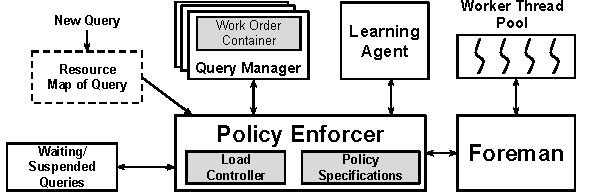
\includegraphics[width=\columnwidth]{figures/Scheduler-Architecture.pdf}
	\vspace*{-1.5em}
	\caption{Overview of the scheduler}
	\label{fig:scheduler-architecture}
	\vspace*{-1.5em}
\end{figure}

An important component of the system is the \textit{Policy Enforcer}.
It selects a query among all the concurrent queries, and schedules its work order for execution. 
This in essence is \textit{a scheduling decision}, and is taken based on a high-level policy provided to the system.
The policy is described in \textit{Policy Specifications}, which is an
abstraction that governs how resources are shared among concurrent queries. 

Policy Enforcer (PE) and various Query Managers (QM) communicate with each other as follows:
\textbf{QM}$\rightarrow$\textbf{PE}: Provide work orders of the managed query for dispatching them for execution.
\textbf{PE}$\rightarrow$\textbf{QM}: Upon every work order completion, send a signal so that the QM can then decide if new nodes in the DAG can be activated, and if existing nodes can be marked as completed.
A detailed description of the Policy Enforcer is present in Section~\ref{ssec:policy-enforcer}. 

The Policy Enforcer contains a \textit{Load Controller} module, which is
responsible for ensuring that the system has enough resources to meet the
demands.
A new query in the system presents its resource requirements for its lifetime in the form of a \textit{Resource Map} to the Load Controller.
%The estimates provided in the Resource Map can come from the query optimizer or some other mechanism, which is irrelevant to the scheduler.
A sample resource map is presented in Appendix~\ref{apx:resource-map}.

The Load Controller determines the fate of a new query. 
If enough resources are available, it admits the query.
If the system risks thrashing due to the admission of the new query, it can take a number of decisions, including wait-listing the query or suspending older active queries to free up resources for the new query.
%The Policy Enforcer maintains queues for wait-listed and suspended queries as shown in Figure~\ref{fig:scheduler-architecture}.
We describe the Load Controller in Section~\ref{ssec:load-control-mech}.

The Policy Enforcer works with another module called the \textit{Learning Agent}. 
Execution statistics of completed work orders are passed from the Policy Enforcer to the Learning Agent.
This component uses a simple learning-based method to predict the time to 
complete future work orders using the execution times of finished work orders. 
Such predictions form the basis for the Policy Enforcer's decisions regarding scheduling the next set of work orders. 

%Work orders that are ready to execute are sent to a \textit{Foreman} module. 
%The Foreman simply acts as a link between the overall scheduler and a pool of 
%worker threads. 
The \textit{Foreman} module acts as a link between the Policy Enforcer and a pool of worker threads. 
It receives work orders that are ready for execution from the Policy Enforcer, and dispatches them to the worker threads. 
The Foreman can monitor the number of pending work orders for each worker, and 
use that information for load-balancing when dispatching work orders.
Upon completion of the execution of a work order, a worker sends execution statistics to the Foreman, which are further relayed to the Policy Enforcer.
New work orders due to pipelining are generated similarly (these details are presented in Appendix~\ref{apx:pipelining}).

\sys{} has two kinds of threads -- a \textit{scheduler} thread and many \textit{worker} threads that perform the actual relational operations as defined by \textit{work orders}. 
More details about the thread model can be found in Appendix~\ref{apx:thread}.

\subsection{Policy Enforcer}\label{ssec:policy-enforcer}
The Policy Enforcer assigns a probability value to each active query in the system. 
The scheduling decisions are taken based on these probabilities. 
A probability value assigned to a query indicates the likelihood of a work order from that query being scheduled. 
The manner in which these probability values assigned to the queries are adjusted helps enforcing the policy. 
The formulations of these probabilities for various policies are expressed in Section~\ref{sec:policy}.

An important information for determining such a probability value is the estimate about the run times of future work orders of the query.
Using these estimates for all the active queries, the Policy Enforcer can tweak the resource allocation to queries with the goal of adhering to the specified policy for resource sharing. 
In the next section, we describe the technique that we use to estimate the execution time of future work orders of a query.
%%Second, what happens if the future execution time of work orders keep changing? 
%Why should we compute the probability using future work order execution times instead of assigning fixed probabilities to queries?
%We answer these questions by introducing a Learning agent module next. 
%In the beginning of a workload execution, the Policy Enforcer uses some default 
%probability values until the Learning Agent collects enough data so as to make a prediction. 
\subsection{Learning Agent}\label{ssec:learning}
The Learning Agent module is responsible for predicting the execution times of the future work orders for a given query. 
It gathers the history of executed work orders of a query and applies a prediction model on such a history to estimate the execution time of a future work order.
This predicted execution time is used to compute the probability assigned to each query (cf. Section~\ref{sec:policy} for probability derivations).

An alternative to the Learning Agent could be a static method that assigns fixed probability values to active queries in the system. 
We now justify the need for the Learning Agent and highlight the limitations of the alternative mentioned above.
An illustrative example is presented in Appendix~\ref{apx:learning-motivation}.

The time per work order metric doesn't stay the same throughout a query's lifetime, for reasons such as variations in input data (e.g. skew), CPU characteristics of different relational operators (e.g. scan vs hash probe).
In each phase of the query, the time per work order is different.
As the query plan gets bigger, the number of phases in the plan increase.
In addition, different queries may be in different phases at a given point in time.
To make things more complicated, queries can enter or leave the system at any time.

Therefore, it is difficult to statically pick a proportion of CPU to allocate to the concurrent queries. 
Hence there is a need to ``learn'' the various phases in the query execution and dynamically change the proportion of resources that are allocated to each query, based on each query's phase.
Next, we study the methodology used by the Learning Agent.
\subsubsection{Learning Agent Methodology}
%The Learning Agent builds each query's \textit{execution profile} based 
%on the execution statistics of recently completed work orders for that query.
The Learning agent uses the execution times of previously executed work orders 
denoted as $t_{w_{1}}, t_{w_{2}}, \ldots, t_{w_{k}}$ to predict the execution time of 
the next work order $t_{w_{k+1}}$ for a given query.\footnote{In the beginning of a query execution, when enough information about work order execution times is not available, we use the default probabilities in the Policy Enforcer, instead of using default predicted times in the Learning Agent.}
Figure~\ref{fig:scheduler-cycle} shows the Learning Agent's interaction with the other scheduler components.
%It receives the execution statistics of an  executed work order, and uses this information 
%to predict the execution time of the future work orders. 

\begin{figure}[]
	\centering
	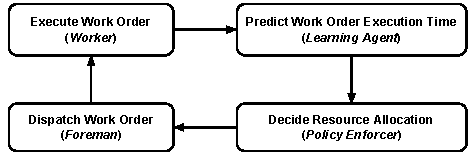
\includegraphics[width=\linewidth]{figures/Compact-SchedulerCycle.pdf}
	\vspace{-2em}
	\caption{Interactions among scheduler components}
	\label{fig:scheduler-cycle}
%	\vspace{-1.5em}
\end{figure}

The set of previously executed work orders can belong to multiple relational operators in the query operator DAG. 
The Learning Agent stores the execution times of the work orders grouped by their source relational operator, e.g. the execution statistics of select work orders are maintained together and kept separate from aggregation work orders. 

%A prediction model is used to estimate the execution time of future work orders. 
\sys{}'s scheduler currently uses linear regression as the prediction model.
We chose linear regression as it is fast, accurate, and efficient w.r.t. the computational and the storage requirements of the model. 
%(New models can be easily added using an abstraction mechanism.) 
More details about our use of linear regression is described in Appendix~\ref{apx:linear-regression-usage}.

We note that the problem of estimating the query execution time is well-studied, but requires complex methods~\cite{duggan2011performance, wu2013towards, li2012gslpi, 
chaudhuri2004estimating}. 
The Learning Agent does not require such methods. 
However, it can combine estimates from other methods with its simple learning-based estimates.
%i.e. we try to predict the execution times of immediate work orders, as opposed  to a 
%global
%level estimation that may involve estimation of the progress of the query and prediction
%of query/workload completion times. The Learning Agent can be extended to use
%other techniques for the prediction, and is complimentary to other methods for
%estimation.
% !TEX root = scheduler.tex
\section{Policy Derivations and Load Controller Implementation}\label{sec:policy}
Our work focuses on two critical system resources for in-memory database deployments: CPU and memory. 
The policies treat CPU as a \textit{divisible resource}, and the policy specifications are defined in terms of relative CPU utilizations of queries or query classes.
The load controller implementation treats memory as a \textit{gating resource} and its goal is to avoid memory thrashing.
We justify the choice of resources for policies and load controller implementations in~\cite{supplement}.

%Next, we present the different policies that are currently implemented in \sys{} to highlight how one can encode policies to work with the probability-based scheduler. 
%As noted above the policies are specified in terms of the CPU resource. 
A policy specification consists of two parts: an inter-class specification (resource allocation policy across query classes), and an intra-class specification (resource allocations among queries within the same class). 
The default setting is uniform allocations for both intra and inter-class policies. 

In Section~\ref{ssec:load-control-mech}, we describe \sys{}'s load control mechanisms. 
The load controller takes admission control and query suspension decisions based on the memory resource.
%These load control mechanisms work in conjunction with the notion of query priority used in the policy implementations.

The scheduling policies, described below in Sections~\ref{ssec:fairness}, ~\ref{ssec:hpf}, and~\ref{ssec:proportional-priority} are subject to the decisions made by the load controller, i.e. the policies apply to the queries that are admitted by the load controller and have not been suspended. %by the load controller. 

%We note that our scheduler framework allows extending the policy implementations and the load control mechanisms to other resource types such as network and disk I/Os, but we defer such extensions to future work, primarily as our implementation is within the context of an in-memory database. 

The interpretations of various policies are presented in Table~\ref{table:policy-interpreatations}.
Note that for the Fair policy, there is only one class. 
For the priority-based policies, we assume that queries are tagged with priority (integer) values. 
%A higher integer implies higher priority. 
Next, we describe the probabilistic framework that we use to implement various policies
(cf. Table~\ref{table:policy-notations} for notations).

\begin{table}[t]
\centering
\begin{tabular}{|p{1.3cm}|p{6.5cm}|}
\hline
\textbf{Policy} & \textbf{Interpretation} \\ \hline
Fair & In a given time interval, all active queries should get an equal proportion of the total CPU cycles across all the cores. \\ \hline%There is only one query class.
Highest Priority First (HPF) & 
%Queries are tagged with priorities and the priority values are ordered. 
Queries are executed in the order of their priority values; i.e. a higher priority query is preferred over a lower priority query for scheduling its work order. \\ \hline
Proportional Priority (PP) & 
%Each query is tagged with a priority value. 
The collective resources that are allocated to a query class (i.e. all queries with the same priority value) is proportional to the class' priority value based on a specified scale; e.g. (linear, exponential).
%in a two class policy, an exponential scale could be used to specify that the high priority class should be given 10 times the resources as the low priority class. 
\\ \hline
\end{tabular}
\caption{Interpretations of the policies implemented in \sys{}}
\label{table:policy-interpreatations}
	\vspace{-2.8em}
\end{table}

\subsection{Fair Policy Implementation}\label{ssec:fairness}
\begin{table}[t]
	\centering
	\begin{tabular}{|p{0.1\columnwidth}|p{0.75\columnwidth}|}
		\hline
		\textbf{Symbol} & \textbf{Interpretation} \\ \hline
		$q_{i}$ & Query $i$ \\ \hline
		$pb_{i}$ & Probability assigned to $q_{i}$ \\ \hline
		$PV_{i}$ & The priority value for $q_{i}$ \\ \hline
		$t_{i}$ & Predicted work order execution time for $q_{i}$ \\ \hline
		$t_{PV_{i}}$ & Proportion of time allocated for the class with priority value $PV_{i}$ \\ \hline
		$prob_{PV_{i}}$ & Probability assigned to the class with priority value $PV_{i}$ \\ \hline
	\end{tabular}
	\vspace{0.4em}
	\caption{Description of notations}
	\label{table:policy-notations}
	\vspace{-3em}
\end{table}

%\textbf{Policy Interpretation}: In a given time interval, all active queries should get an equal proportion of the total CPU cycles across all the cores.
%There is only one query class and the default (i.e. uniform) policy is used for intra-class queries. 
%Thus the collective CPU resource (i.e. all cores across all sockets) is to be shared \textit{equally} by all concurrent queries. 

We assume $k$ concurrent active queries: $q_{1}, q_{2}, \ldots q_{k}$. 
The probability $pb_{j}$ is computed as:
%\begin{displaymath}
%$pb_{j} = \frac{\frac{1}{t_{j}}}{\sum\limits_{i=1}^{k}\frac{1}{t_{i}}}$
%\end{displaymath}
$pb_{j} = (\frac{1}{t_{j}})/(\sum\limits_{i=1}^{k}\frac{1}{t_{i}})$

Observe that $pb_{j} \in (0, 1]$ and $\sum\limits_{j=1}^{k}pb_{j} = 1$. 
Therefore, the $pb_{j}$ values can be interpreted as probability values. 
As all the probability values are non-zero, every query has a non-zero chance of getting its work orders scheduled. 

Notice that $\forall i, j$ such that $1 \leq i, j \leq k$, 
%\begin{displaymath}
%\frac{pb_{i}}{pb_{j}} = \frac{t_{j}}{t_{i}}
%\end{displaymath}
$pb_{i}/pb_{j} = t_{j}/t_{i}$.

If $t_{i} > t_{j}$, it means that the work orders for query $q_{i}$ take longer time to execute than the work orders for query $q_{j}$. 
Thus, in a given time interval, fewer work orders of $q_{i}$ must be scheduled as compared to the query $q_{j}$. %, as depicted in Figure~\ref{fig:probability-explanation}.

The probability associated with a query determines the likelihood of the scheduler dispatching a work order for that query.
Thus, when $t_i > t_j$, $pb_j > pb_i$, i.e.  the probability for $q_{i}$ should be proportionally smaller than probability for $q_{j}$.

\subsection{Highest Priority First (HPF) Implementation}\label{ssec:hpf}
%\textbf{Policy Interpretation}: Queries are tagged with priorities and the priority values are ordered. 
%Queries are executed in the order of their priority values; i.e. a higher priority query is preferred over a lower priority query for scheduling its work order. 
%The intra-class policy is set to the default (i.e. fair to all the queries within the class)
%Queries in the same priority class are all treated equally, i.e. their resource allocation is identical.
%Each query $q_{i}$ is associated with a priority value $pv_{i}$, where $pv_{i}$ is a 
%positive integer. 
Let $\{PV_{1}, PV_{2}, \ldots, PV_{k}\}$ be the set of distinct priority values in the 
workload. 
A higher integer is assumed to imply higher importance/priority.
The scheduler first finds the highest priority value among all the currently active queries 
which is $PV_{max}$. % = max(PV_{1}, PV_{2}, \ldots, PV_{k})$. 
Next, a fair resource allocation strategy is used to allocate resources across all the active queries in that priority class. 

%Note that with the HPF policy, if higher priority queries keep arriving continually, then 
%lower priority queries could starve.

In some situations, the queries from the highest priority value may not have enough work to keep all the workers busy. 
In such cases, to maximize the utilization of the available CPU resources, the 
scheduler may explore queries from the lower priority values to schedule work orders.
\subsection{Proportional Priority (PP) Implementation}\label{ssec:proportional-priority}
%\textbf{Policy Interpretation}: Each query is tagged with a priority value.
%The collective resources that are allocated to a query class (i.e. all queries with the same priority value) is proportional to the class' priority value based on a specified scale; e.g. in a two class policy, an exponential scale could be used to specify that the high priority class should be given 10 times the resources as the low priority class. 
%The intra-class policy is set to the default (i.e. uniform).
Let $P = \{PV_{1}, PV_{2}, \ldots PV_{k}\}$ be the set of the distinct priority values 
in the workload. 
We assume a linear scale for the priority values. 
A higher integer is presumed to imply higher priority.

In a unit time, a class with priority value $PV_{i}$ should get resources for a time that is 
proportional to its priority value i.e. $PV_{i}$. 
Therefore, the class with priority $PV_{i}$ should be allocated resources for 
$t_{PV_{i}} = PV_{i}/\sum\limits_{j = 1}^{k}PV_{j}$ amount of time. 

We now estimate the number of work orders for priority class $PV_{i}$ that can be executed in its allotted time. 
For this task, we need an estimate for the execution time of a future work order from the class as a whole, referred to as $w_{PV_{i}}$ for the class with priority value $PV_{i}$.
Therefore, assuming $m$ queries in a given class and the individual estimates of 
work order execution times for queries with priority $PV_{i}$ are $t_{1}, t_{2}, \ldots, t_{m}$, then the predicted work order execution time for the class is $w_{PV_{i}} = \sum\limits_{j = 1}^{m}t_{j}/m$.
Therefore the estimated number of work orders executed for priority class $PV_{i}$ is
$n_{PV_{i}} = t_{PV_{i}} / w_{PV_{i}}$.

After determining $n_{PV_{1}}, n_{PV_{2}}, \ldots, n_{PV_{k}}$, which are the 
estimated number of work orders executed by all the priority classes in their allotted
time, computing probabilities for each class is straightforward.
The probability of priority class $PV_{i}$ is 
$prob_{PV_{i}} = n_{PV_{i}}/\sum\limits_{j = 1}^{k}n_{PV_{j}}$

Next, we describe the load control mechanism. % in \sys{}.
\subsection{Load Control Mechanism}\label{ssec:load-control-mech}
As described earlier, the load control mechanism in \sys{} is designed to manage the availability of memory resource to the queries in the system.
This task requires continuous monitoring of memory consumption in the system.
The load controller component has two functions:
1) Determining if new queries are allowed to run (a.k.a. admission control).
2) Suspending queries if the system is in danger of thrashing.
We now explain how the load control mechanism realizes these two functions.

%In this section we describe some example load control mechanisms implemented in \sys{}.

Recall from Section~\ref{sec:design}, that a new query entering the system presents to the Load Controller its Resource Map that describes the query's estimated range of resource requirements.

We denote the minimum and maximum memory requirements for a given query as $m_{min}$ and $m_{max}$, the threshold for maximum memory consumption for the database as $M$ and the current total memory consumption as $m_{current}$. 
The term $m_{current}$ includes total memory occupied by various tables, run time data structures such as hash tables for joins and aggregations for all the queries in the system.

In the simplest case, when there is enough memory to admit the query, we have $m_{max} + m_{current} < M$. 
In this case, the load controller can let the query enter the system.

When memory is scarce, i.e. $m_{min}+m_{current}>M$, the query can not be admitted right away. 
Its admission depends on the system's policy (i.e. one of the policies described earlier).

If the system is realizing the fair policy, all queries have the same priority.
In this scenario, the load controller simply suspends the new query until enough memory becomes available, after which the query can be admitted.

For both priority-based policies, if the new query's priority is smaller than the minimum priority value in the system, then the load controller suspends the query. 
The suspended query can be admitted in the system when enough memory is available to admit it.
In the other case, the load controller finds queries from the lower priority values that have high memory footprints. 
It continues to suspend such queries from the lower priority levels (in decreasing order of memory footprints) until enough memory becomes available to admit the given query. 

%The load control mechanism can also be used continually to monitor the actual memory consumption of queries, and suspend existing queries if the actual memory consumption ($m_{current}$) approaches a pre-defined threshold limit.
%The decisions made by the load controller are logged, so that its actions can be viewed in a control dashboard.
% performs admission control for all the policies. In the future, the load controller can be made to monitor run--time memory allocations and with the help of the \sys{}'s buffer pool, control such allocations requested by queries in the system.
%or equal to the currently running queries in the system, the Load Controller may waitlist the query.
%However, if the new query has a higher priority than the currently running queries in the system, it can decide to make memory available for the query, so as to admit it.
%One possible way to free up the memory is by suspending existing queries in the system in decreasing order of their memory footprints, until there is enough memory available to let the new query in the system.
%The suspended queries can be reactivated when there are enough resources available to execute them. 
% !TEX root = scheduler.tex
\section{Evaluation}\label{sec:eval}
We present an evaluation of our scheduler in this section. 
The goals of the experimental evaluation are as follows:
\begin{enumerate}
%\itemsep -0.1em
\item To check whether the policy enforcement meets the expected criterion defined in 
the policy behavior. 
\item To illustrate the role of the learning component, we compare with a static implementation of policies that doesn't use the learning-based feedback loop. 
The probabilities assigned to each query in such implementation are statically determined and they do not change.
\item Examine the behavior of the learning-based scheduler in the presence of 
execution skew. 
\item To check how the load balancing component of the scheduler works in extreme/overloaded scenarios.
\end{enumerate}
\subsection{Evaluation Platform}
In this section, we describe the hardware used for our experimental evaluation. 

We use a machine %provided by the CloudLab~\cite{RicciEide:login14} service for the experiments.
that has two Intel Xeon Intel E5-2660 2.60 GHz (Haswell EP) processors. 
Each processor has 10 cores and 20 hyper-threading hardware threads. 
The machine runs Ubuntu 14.04.1 LTS. 
It has a total of 160 GB ECC memory with 80 GB of directly-attached memory per NUMA socket. 
Each processor has a 25 MB L3 cache shared by all of its cores. 
Each core has a 32 KB L1 instruction cache, 32 KB L1 data cache, and a 256 KB L2 cache.
%This machine has two 1.2 TB 10K RPM SAS HDDs, and one 480 GB SAS SSD device.
\subsection{\sys{} Specifications}
We now describe \sys{}'s configuration parameters used in the experiments. 
\sys{} uses all 40 threads in the system as worker threads.
Each worker thread is pinned to a CPU core. 
Such pinning prevents migration of a thread from one CPU core to another by the OS, which may incur cache misses and migration penalties.
The scheduler thread is not pinned, as its CPU utilization is low and it is not worth dedicating a CPU core for the scheduler thread.

\sys{}'s buffer pool is configured with 80\% of the available system memory (126 GB). 
Memory for storage blocks, temporary tables and hash tables is allocated from the buffer 
pool.
The block sizes for all the stored relation is set to 4 MB.
We preload the buffer pool before executing the queries, which means that the queries run 
on ``hot'' data. 

To encode the priority information in a query, we modify \sys{}'s SQL parser.
The example below shows a query with priority value as 2:
\lstset{language=SQL, 
	basicstyle=\ttfamily\footnotesize, 
	showstringspaces=false,
	keywordstyle=\color{cardinal}\bfseries, 
	otherkeywords={WITH, PRIORITY},
	emph=[1]{San,Diego}, emphstyle=[1]{\color{bondiblue}}}
\begin{lstlisting}
SELECT * FROM Employees WHERE salary > 90000 WITH PRIORITY 2;
\end{lstlisting}
\vspace{-1em}

\subsection{Experimental Workload}\label{ssec:workload}
For our experimental evaluation, we use the Star Schema Benchmark (SSB)~\cite{ssb}. 
%The SSB is based on the TPC-H benchmark, and is designed to measure the query performance when %database systems in support of classical 
%the data warehouse uses the popular Kimball~\cite{Kimball} approach. 
%At a scale factor of X, the benchmark corresponds to about X GB of data in the 
%corresponding TPC-H warehouse.
The SSB benchmark has 13 queries, divided in four categories. 
%Each query is identified as \textbf{qX.Y}, where $X$ is the class and $Y$ is the query 
%number within the class.
%There are four query classes. 
%, i.e. $1\leq X\leq4$. 
%The first and second classes have three queries each, the third class has four queries, and 
%the fourth class has three queries.
The queries in each category are similar with respect to aspects such as the 
number of joins in the query, the relations being joined, the filter and aggregation 
attributes. 
The grouping of queries in various classes makes this benchmark suitable for our 
experiments, as it provides a way of assigning priorities to the queries based on their class. 

%The dataset has 1 fact and 4 dimension tables. 
We use SSB SF 100 dataset in two ways -- uniform and skewed distribution. 
%first, we generate uniform data in all the relations as per the  original benchmark specification~\cite{ssb}.
We introduce skew in the \textit{lo\textunderscore quantity} column of \textit{lineorder} table, as described by Seelam et al.~\cite{DBLP:conf/wosp/2013}.
% with the values derived from a probability distribution function: $ P(X=x) = (0.3/1.3^{x})$. 
%The range of values in \textit{lo\textunderscore quantity} column is $[1, 50]$. 
In the uniform dataset, every value in the domain [1, 50] is equally likely to appear in the \textit{lo\textunderscore quantity} column.
The skewed version, 90\% values belong to the range $[1, 10]$. 

\subsection{Evaluation of Policies}\label{ssec:policy-eval}
In this section, we evaluate various policies currently implemented in the system.
All the policies are specified in terms of the CPU resources. 
With these experiments, we verify if the actual CPU allocation among queries is in accordance with the policy specifications.
To calculate CPU utilization, we log the start and end times for each work order and use this log to calculate the CPU utilization.
%we extract all event points whenever a work order starts or ends. We aggregate how many workers that each query is assigned to between two consecutive event points. Later on, we group them into fixed size intervals (e.g N1 ms) and calculate average number of workers that the query has in these intervals. We normalize the number of workers that each query has by dividing all values to total number of workers in the system. For plotting purpose, the values are smoothed by using rolling average over N2 consecutive window values.
%\reminder{Give values for N1 and N2}

\subsubsection{Fair}
In this experiment, we execute all 13 queries from the SSB concurrently using the fair policy. 
As described in Section~\ref{ssec:fairness}), the policy specification implies a fair sharing of CPU resources among concurrent queries.
The CPU utilization of the queries is depicted in Figure~\ref{fig:fair-cpu-util}.
As we can see, %from Figure~\ref{fig:fair-cpu-util}, 
the CPU utilization of all the queries remains nearly equal to each other during the workload execution, despite queries belonging to different query classes with varying query complexities.

\begin{figure}[]
	\centering
	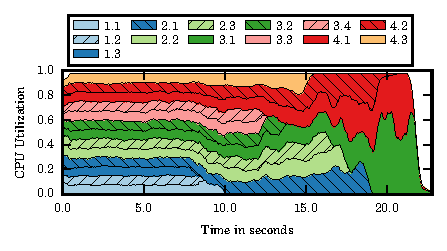
\includegraphics[width=\columnwidth]{figures/ssb-all-uniform-fair-cpu-util.pdf}
	\vspace{-2.5em}
	\caption{CPU utilization of queries in fair policy}
	\label{fig:fair-cpu-util}
\end{figure}

Notice that the available CPU resources also get automatically distributed elastically among the active 
queries (e.g. at the 10 and 15 seconds marks) when a query finishes its execution. 
This elasticity behavior allows \sys{} to fully utilize the CPU resources at \textit{all} times.
\subsubsection{HPF}
In this experiment, we validate whether the implementation matches the policy 
specification of HPF (Highest Priority First, cf. Section~\ref{ssec:hpf}),
which requires that when scheduling work orders, higher priority classes be 
preferred over lower priority classes. 

\begin{figure}[b]
	\centering
	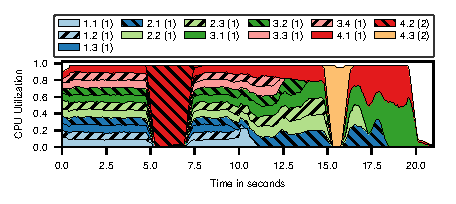
\includegraphics[width=\columnwidth]{figures/ssb-hpf-all.pdf}
	\vspace{-2.5em}
	\caption{CPU utilization in HPF policy. Note that $a.b  (N)$ denotes a SSB query $a.b$ with priority $N$}
	\vspace{-1em}
	\label{fig:hpf-all}
\end{figure}

As before, we use all the 13 SSB queries for this experiment. 
In this experiment, the first 11 queries from the benchmark have the same priority value (1).
The last two queries (Q4.2 and Q4.3) are given a higher priority value (2). 
The execution begins with the first 11 queries in the benchmark, i.e. Q1.1 to Q4.1.

We inject Q4.2 in the system at around 5 seconds and Q4.3 at around 15 seconds.
Figure~\ref{fig:hpf-all} shows the CPU utilization of queries during the workload 
execution.

Note that when the high priority queries arrive (at the 5 and 15 seconds marks), the existing queries pause their execution and the scheduler makes way for the higher priority query.
As soon as a higher priority query finishes its execution (i.e. at the 7 and 16 seconds marks), other low priority queries simply resume their execution.

The result of this experiment shows that \sys{}'s scheduler design naturally supports 
query suspension, which is an important concern in workload management. 

\subsubsection{Proportional Priority}\label{sssec:pp-policy-exp}
The goal of this experiment is to verify the scheduler's behavior to the proportional priority policy (cf. 
Section~\ref{ssec:proportional-priority}).
In this policy, the CPU allocation to query classes should be in accordance to their priority values.

We pick two queries from each SSB class, and assign them a priority value. 
The priorities assigned to the queries are based on the query complexity of their corresponding query class. 
For instance, query class 1 has only one join, class 2 has two joins and so on.
Recall that in our implementation a higher priority integer implies higher importance cf. 
Section~\ref{ssec:proportional-priority}.

Figure~\ref{fig:pp-cpu-util} shows the CPU allocation among concurrent queries in the proportional priority policy.
We can see that a higher priority query gets proportionally higher share of CPU as 
compared to the lower priority queries.
When all queries from the priority class 8 finish their execution (11 seconds), the 
lower priority classes elastically increase their CPU utilization, so as to use all the CPU 
resources. 
Also note that among the queries belonging to the same class, the CPU utilization is 
nearly the same, as described in the policy specifications.

\begin{figure}[]
	\centering
	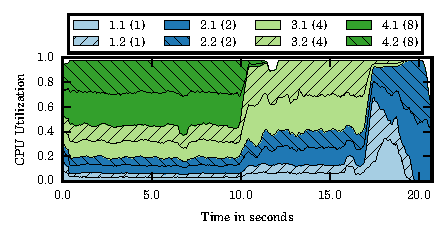
\includegraphics[width=\columnwidth]{figures/ssb-priority-uniform-2queries-perclass-cpu-util.pdf}
	\vspace{-2.5em}
	\caption{CPU allocation for proportional priority policy. Note that $a.b  (N)$ denotes a SSB query $a.b$ with priority $N$}
	\label{fig:pp-cpu-util}
	%	\vspace{-1em}
\end{figure}


\subsection{Impact of Learning on the Relative CPU Utilization}\label{ssec:learning-impact-cpu-util}
In this experiment, we compare the learning-based scheduler implementation with a 
non-learning based implementation (baseline).
We perform the comparison using fair policy, which should be the easiest policy for a static method to realize.

In the baseline, the probability assigned to each query remains fixed unless either a query is added or removed from the system.
If there are $N$ active concurrent queries in the system, each query is assigned a probability $1/N$.
%In the proportional priority implementation, if the distinct priority levels are $p_1, p_2 
%\ldots p_k$, then priority $p_i$ gets a probability $\frac{p_i}{\sum\limits_{j = 
%0}^{k} 
%p_j} $.

We run $Q1.1$ and $Q4.1$ together with the fair policy in both the learning and 
non-learning implementations.
Our metric for this experiment is the ratio of CPU utilizations of $Q4.1$ and $Q1.1$.
%The CPU utilization is calculated as explained in Section~\ref{ssec:policy-eval}.
As per the policy specifications, the CPU utilization for both queries in the fair policy 
should be equal. % to each other, which means the ideal ratio is 1.
Figure~\ref{fig:non-learning-comparison} shows the results of this experiment.
%We restrict the X-axis until both the queries are under execution. 

\begin{figure}[t]
	\centering
	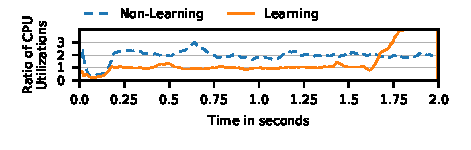
\includegraphics[width=\columnwidth]{figures/q1-q11-ratio-cpu-util.pdf}
	\vspace{-2em}
	\caption{Ratio of CPU utilizations  $\frac{Q4.1}{Q1.1}$ for learning and non-learning 
		implementations}
	\label{fig:non-learning-comparison}
	\vspace{-1.5em}
\end{figure}

Observe in Figure~\ref{fig:non-learning-comparison}, that the ratio in the non-learning implementation is closer to 2, meaning that the 
implementation is biased towards $Q4.1$. 
Recall from Figure~\ref{fig:q1.1-q4.1-time-per-wo} that the time per work order for $Q4.1$ is higher than $Q1.1$. 
In contrast, the ratio of CPU utilizations in the learning implementation is nearly 1.
The learning based implementation can identify various phases in query execution for 
both the queries and adaptively change the CPU allocation as per the changing demands 
of the queries.
The non-learning implementation however fails to recognize the fluctuations in the CPU 
demands of queries and therefore does an unfair allocation of CPU resources.
%\subsubsection{Impact of Learning on Performance}\label{sssec:makespan-comparison}
%To gauge the impact of the learning on performance, we compare the makespan (i.e. the total execution time of the entire workload) in learning vs non-learning implementations.
%For this comparison, we again use the fair policy, as earlier. 
%%in the experiment described in Section~\ref{ssec:learning-impact}.
%Table~\ref{table:makespan-learning-vs-non-learning} describes the results of the experiments using two workloads using the makespans using learning and non-learning implementations.  
%
%We can observe that the overhead of learning is negligible, in fact it benefits the makespan of the SSB workload by around 11\%, as compared to the non-learning implementation. 
%This improvement is due to a ``fairer'' allocation of CPU resources to the queries in the learning implementation.
%Longer queries don't dominate the CPU resource consumption, because of which shorter queries can finish their execution sooner.
%, thereby freeing up CPU resources available for the longer queries, which in turn can finish execution faster.
%\begin{table}
%\centering
%\begin{tabular}{|c|l|l|}
%\hline
%\multirow{2}{*}{Workload} & \multicolumn{2}{c|}{Makespan (sec)} \\ \cline{2-3} 
% & Non learning & Learning \\ \hline
%Q1.1 and Q4.1 & 4.2 & 4.3 \\ \hline
%All SSB queries & 25.6 & 22.9 \\ \hline
%\end{tabular}
%\vspace{0.5em}
%  \caption{Makespan comparison of learning and non-learning implementation}
%  \label{table:makespan-learning-vs-non-learning}
%\end{table}
%We would like to stress that the primary goal of the learning implementation is to aid the scheduler to adhere to the high level policy. 
%These experiments %described in Section~\ref{ssec:learning-impact} and Section~\ref{sssec:makespan-comparison} 
%suggest that the learning implementation not only achieves its primary goal, but also helps improving the performance of the SSB workload. 
\subsection{Impact of Learning on Performance}\label{ssec:learning-impact-perf}
In this experiment we analyze the impact of the learning-based approach on the performance of queries. 
We use the same setup as the previous experiment and begin the execution with 10 queries; with five instances each of $Q4.1$ and $Q1.1$ running concurrently. 
As soon as one instance of $Q4.1$ finishes its execution, another instance of $Q4.1$ enters the system (likewise for $Q1.1$).
We compare the throughput for both $Q4.1$ and $Q1.1$ using the learning implementation of the fair policy against its non-learning implementation.

%In real life workloads, there is often a mix of queries with different query execution times.
%Based on this setting, we assume two users of the database system issuing concurrent queries. 
%One user issues short running queries and another user issues longer running queries. 
%\sys{} runs both kinds of queries concurrently using fair policy. 

%We compare the throughput observed by both users in the learning-based fair policy with non-learning based fair policy implementation, at the end of \reminder{add time} minutes from the beginning of the workload execution. 
%The concurrent query execution begins with \reminder{add number} queries, \reminder{add number} from each user.
%As soon as a user is returned the result of a query, the same user issues the next query to \sys{}, which means the think time is 0. 

%Table~\ref{table:throughput-comparison} compares the throughput observed by the two users. 
%We can observe that the throughput for the user issuing longer queries is less impacted by the change in the policy implementation. 
%However, the user issuing shorter queries is highly benefited using a learning based implementation.
%The throughput is nearly \reminder{add number}X better in the learning implementation compared to the non-learning one. 
Figure~\ref{fig:q11-q41-throughput} plots the result of this experiment and shows the throughput for each query ``stream''. 
The throughput for the $Q4.1$ stream is not affected considerably by the choice of the implementation. 
However the throughput of the $Q1.1$ stream is improved significantly using the learning implementation, and it is upto 3x better than the throughput using the non-learning implementation. 
The reasons for the improvement are as follows:
Following the result of the previous experiment (cf. Figure~\ref{fig:non-learning-comparison}),
in the non-learning implementation, $Q1.1$ which has shorter work orders, gets starved of CPU resources due to $Q4.1$, which has longer duration work orders. 
In the learning-based implementation however, the $Q1.1$ stream gets its fair share of CPU resource (more than that in the non-learning implementation). 
Therefore, $Q1.1$'s performance is improved, resulting in its increased throughput. 

This experiment highlights a two-fold impact of the learning module -- first, it plays a crucial role in the fair policy enforcement. 
Second, it improves performance of queries with lower CPU requirements when they are competing with queries with higher CPU requirements, thereby also increasing overall system throughput with such mixed and diverse workloads. 

\subsection{Experiment with Skewed Data}
In this experiment we test the learning capabilities of the \sys{} scheduler under the presence of skew. 
We introduce skew in the dataset as described in Section~\ref{ssec:workload}, and once again execute $Q1.1$ and $Q4.1$ on the skewed dataset.
We sort the skewed \textit{lineorder} table on the \textit{lo\textunderscore quantity} column, so that the impact of skew is amplified, i.e. on the data blocks when the predicate $lo\textunderscore quantity \leq 25$ is evaluated, very few tuples are selected for some blocks, and for other blocks a large number of tuples are selected.

\begin{figure}[t]
	\centering
	\subfigure[$Q1.1$]{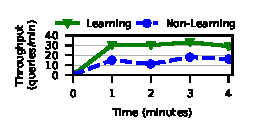
\includegraphics[]{figures/q11-throughput.pdf}}
	\subfigure[$Q4.1$]{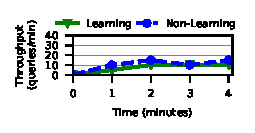
\includegraphics[]{figures/q41-throughput.pdf}}
	\vspace{-0.6em}
	\caption{Impact of learning on the throughput}
	\label{fig:q11-q41-throughput}
	\vspace{-1em}
\end{figure}
	
To test the scheduler's ability to learn in the presence of skew, we perform a comparison between the predicted work order times for each query against the observed work order times for the same query.
For completion, we perform the same experiment on the skewed data and uniform data. Figure~\ref{fig:pred-vs-observed-time-per-wo} presents the results of this experiment, with relative error of the prediction on the Y-axis and time on X-axis.
We can see that the relative error is very low in both the uniform and the skewed dataset for both queries. 
Due to the skew, $Q1.1$ takes more time as compared to the uniform dataset.
The intermediate peaks in the relative error correspond to phase change in the execution plan. 
Note that the scheduler learns the phase changes quickly, and adjusts its estimates after each phase change. 

\begin{figure}[b]
	\centering
	\subfigure[Skewed dataset]{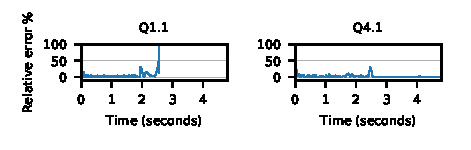
\includegraphics[]{figures/q11-q41-prediction-accuracy-skew-data.pdf}}
	\subfigure[Uniform dataset]{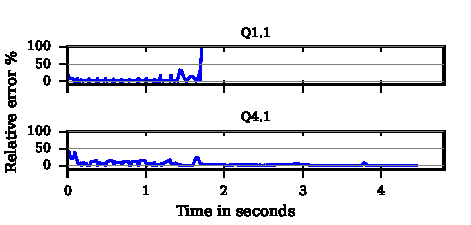
\includegraphics[]{figures/q11-q41-prediction-accuracy-uniform-data.pdf}}
	\vspace{-1em}
	\caption{Comparison of predicted and observed time per work order}
	\label{fig:pred-vs-observed-time-per-wo}
	\vspace{-1em}
\end{figure}

\subsection{Load Control}
The setup for this experiment is the same as that described in Section~\ref{sssec:pp-policy-exp}.
%The buffer pool however is sized down to 70 GB, in order to create an environment 
%of memory pressure.
We set the load controller policy to specify that the threshold for suspending queries is 56 GB, which means that as soon as the buffer pool size grows close to the threshold, the load control mechanism kicks in.

\begin{figure}[t]
	\centering
	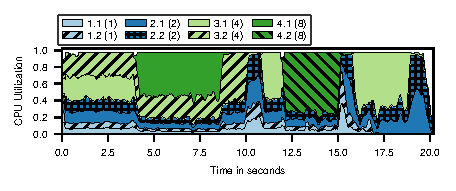
\includegraphics[width=\columnwidth]{figures/load-control-cpu-util.pdf}
	\caption{Load control: An SSB query $a.b$ with priority $N$ is denoted as $a.b (N)$}
	\label{fig:load-control-cpu-util}
\end{figure}

%Recall from Section~\ref{sec:background} that the 
\sys{}'s buffer pool stores not just the tables but also hash tables used for joins and aggregations.
%The LRU-k based buffer pool implementation may evict cold pages if there is a need to make more memory available.
If the requested memory can't be allocted within the memory limits, the load controller 
can suspend a query with the highest memory footprint. 
In the current implementation, the check for reactivating the suspended query is performed upon every query completion and it involves similar memory considerations as that described above. 
Figure~\ref{fig:load-control-cpu-util} shows the CPU utilization of the queries.

The execution begins with 2 queries each from the classes with priority values 1, 2 and 4.
At around 4 seconds, a high priority query $Q4.1$ enters the system.
At this point $Q3.1$ has the highest memory footprint and the load controller
picks it as the victim for suspension.
We can observe in Figure~\ref{fig:load-control-cpu-util}, that in the region between 4
and 11 seconds, the CPU utilization of $Q3.1$ drops down to zero, thus
reflecting its suspended state.

The same pattern is repeated as we inject another high priority $Q4.2$ at around 12 seconds.
Once again $Q3.1$, that has the highest memory footprint, is suspended in order to allow $Q4.2$ to enter the system. 
In Figure~\ref{fig:load-control-cpu-util}, we can observe that in the 12-15 s time interval, $Q4.2$ finishes its execution and the suspended $Q3.1$ doesn't utilize any CPU resource.

This experiment demonstrates the load control capabilities of the \sys{}
scheduler. 
It stresses an important feature of our scheduler, which integrates load-controller functionality. %closely with the resource allocation components, 
Thus, admission control and query suspension is handled holistically by the scheduler. 
% !TEX root = scheduler.tex
\section{Related Work}\label{sec:related}
We now describe the related work on scheduling in database systems, operating systems (OS), and networks. %, and cluster computing. 

The \textit{work orders} abstraction is similar to other abstractions like \textit{morsels} in Hyper~\cite{morsel} and the \textit{segment-based parallelism}~\cite{wang2016elastic}. 
Such abstractions provide a means to achieve high intra-query, intra-operator data parallelism.
Hyper~\cite{morsel} uses a \textit{pull-based} scheduling approach i.e. workers \textit{pull} work (morsels) from a pool.
%Every worker thread continues to pull a morsel from a global pool, and executes it.
We use a \textit{push-based} model, where the scheduler controls the assignment of work to workers.
The pull-based dispatch model suffices for executing one query at a time. 
However, a push-based model can be simpler to implement sophisticated functionalities such as priority-based query scheduling, incorporating a flow control across multiple pipelines, (as shown in~\cite{wang2016elastic}), cache-conscious task scheduling.

The elastic pipelining implementation~\cite{wang2016elastic} uses a \textit{scalability vector} to vary the degree of parallelism of segments of the query plan.
The scalability vector tracks the query performance when number of cores are varied,  and it does not use any prediction technique.
Their objective is to maximize the performance of a single query executed on a cluster.
Our work focuses on resource sharing among concurrent queries, by enforcing policies using a learning-based approach. 
Additionally, we can accommodate estimates provided by other techniques.

There is related work~\cite{gupta2009fair} on ordering queries in a workload with different objectives such as fairness, effectiveness, efficiency and QoS. 
This work is complimentary to our scheduler design as it deals with ordering the queries \textit{before} they enter the system, where as we focus on scheduling \textit{admitted} queries. 
%\textit{Qshuffler}~\cite{ahmad2011interaction} is a query 
%scheduler for report generation workloads. 
%It clusters queries based on their interaction with each other and predicts the 
%performance of the mix using statistical methods.
%It does not preempt queries once they are scheduled, whereas \sys{}'s 
%scheduler uses fine grained control over query execution, allowing query suspension and resumption. 

%In business intelligence settings, workload management is an important challenge.
%Some techniques to manage workloads are based on QoS considerations. 
%Krompass et al.~\cite{krompass2007dynamic} identify and handle mis-behaving queries in a workload, and also propose an economic model for prioritizing and penalizing queries based on their service level agreements~\cite{krompass2006quality}.
%Such techniques can be combined with our scheduler. 
%For instance, our load-controller's action on a query that uses large amount of memory is to suspend it. 
%Alternate actions could be to re-prioritize, kill, or resubmit the query, as described in~\cite{krompass2007dynamic}.
%\sys{}'s prioritized query execution approach can be effective in  scenarios involving 
%SLAs. 

Several enterprise databases~\cite{res_gov, rm, DB2, teradatawm, gpdb, hpwm} offer
workload management solutions which %such as admission control capabilities, 
classify queries based on their estimated resource requirements % (e.g. CPU, memory, I/O), 
encode resource allocation limits as resource pools and map workloads to such resource pools. 
While such estimation methods can be used to complement our approach, 
our scheduler can also work without such detailed estimation techniques. 
Prior research in this area~\cite{krompass2007dynamic, krompass2006quality} has focused on identifying misbehaving queries, prioritizing/penalizing queries to meet the service level objectives.
Our load controller can be complemented with such functionalities.

%Resource (particularly memory) management, is a crucial problem for database systems. 
%Prior work in this area~\cite{mehta1993dynamic, davison1995dynamic} has focused on dynamic memory allocation schemes.
%Mehta and Dewitt's~\cite{mehta1993dynamic} memory allocation scheme
%grouped queries by their estimated memory requirements, and allocated memory to different query classes. 
%Davison and Graefe introduced a resource brokering model~\cite{davison1995dynamic} to minimize query execution times with a constraint of fairness.
%These techniques are complimentary to our execution engine and can also be incorporated in our buffer manager. 

Predicting query performance is an active area of research. 
Earlier work~\cite{wu2013towards, wu2014uncertainty, duggan2011performance} includes analytical model based on the optimizer's cost models for both single query and multiple concurrent queries.
By design, our Learning Agent can incorporate such techniques, but can also function without them. 
More accurate work order execution time estimates can further improve adherence to the policy specifications.
%Wu et al.~\cite{wu2013towards, wu2014uncertainty} developed an analytical model using optimizer's cost model to estimate the CPU and I/O costs for individual query, and used a queueing model to estimate the execution times of concurrent queries in a workload.
%Duggan et al.~\cite{duggan2011performance} presented a model to estimate the performance impact of running concurrent queries.
%Our Learning Agent's prediction accuracy can benefit from such models, 
%Despite these advances in the area of execution time estimation, using 
%inaccurate estimates for achieving fairness may result into unfair schedules. 

%There is a significant interest in minimizing workload execution time by sharing 
%data and computations across queries.
%QPipe~\cite{harizopoulos2005qpipe} exploits common data and operations among 
%different queries. 
%CJoin~\cite{candea2009scalable} operator introduced by Candea et al. continuously 
%scans the fact table, applies predicates from different queries and routes the 
%results to individual queries.
%Zukowoski et al. proposed \textit{co-operative scans}~\cite{zukowski2007cooperative} 
%to share scan operations among concurrent queries. 
%%The sharing of scans reduces the number of I/O operations, increases the data 
%%sharing among concurrent queries thereby improving the latency of individual 
%%queries and the overall execution time. 
%SharedDB~\cite{giannikis2012shareddb} creates a single global query plan for a 
%workload to share computations across queries, thus making it suitable for high 
%throughput demanding environments. 
%These sharing approaches treat every query equally and it is not clear if they 
%can respect query priorities.
%Work and data sharing in \sys{} can be achieved by changing the way work orders are
%created, e.g. if multiple queries need to scan the same block, a single work order can
%be created for all of them. 
%In practice, we create separate work orders for different queries to keep the 
%execution simple.
%Additionally, many database systems \reminder{Can we use examples of Postgres, 
%Greenplum, SQL server, Oracle here?} still follow the \textit{query-at-a-time} 
%model.
%In such systems, our scheduler paves a way towards policy-driven execution
%of concurrent queries. 

Scheduling problem has also been studied in the OS and the networks community. 
%Kay and Lauder~\cite{kay1988fair} described \textit{Share}, a pioneering scheduler that ensured fairness for all the system users.
Our scheduler's probabilistic framework is inspired by the seminal lottery scheduling~\cite{lottery-scheduling} % by Waldspurger and Weihl,
in which different processes are assigned certain number of lottery tickets,
A lottery is conducted after every fixed time intervals and the winner process gets to execute in the next quantum. 

A key difference in lottery scheduling and our work is that the OS scheduling is usually preemptive. %, meaning that a process can be preempted after it uses its time slice. 
The OS maintains a process context that captures the state of the preempted process. 
\sys{}'s scheduling is non-preemptive, which means once a work order begins its execution on a CPU core, it continues to do so until completion.
Non-preemptive scheduling provides us an exemption from maintaining work order context (similar to process context), thereby simplifying the relational operator execution algorithms.
execution time
%\reminder{Removed OS refs}
%Meehan~\cite{meehean2011towards} analyzed various Linux CPU schedulers, %like O(1), CFS, and BFS. 
%showcased the issues of black box CPU scheduling and highlighted the need for increased transparency in CPU scheduling.
%%It achieves fairness by assigning equal proportion of time to the users and not 
%%to the individual processes that are running on the system. 
%%Pabla et al.~\cite{pabla2009completely} described how the Completely Fair Scheduler (CFS) strives to be fair to all the processes running in the Linux. 
%Peter et al.~\cite{peter2010design} proposed design principles for multi-core schedulers used in general purpose OS.
%Giceva et al.~\cite{giceva2013cod} advocated co-designing database and OS for their better integration.

\sys{}'s scheduler design aligns to the idea that scheduling must be transparent, fine-grained, and most importantly the need to separate mechanisms from policies~\cite{LampsonS76} - a common theme found in the OS literature.

Deficit Round Robin (DRR)~\cite{shreedhar1996efficient} is a technique for network packet scheduling.
Our usage of work order execution time as a metric is similar DRR's usage of packet sizes. 
However DRR scheduling is inherently round robin based (with additional maintenance of quantum information), where as our scheduling is based on dynamic probabilities. 

%\reminder{Removed cluster scheduling refs}
%Cluster scheduling has received a wide attention recently.
%Isard et al.~\cite{isard2009quincy} encoded the problem of scheduling jobs on compute nodes in the cluster as a graph that captures the data-locality and fairness requirements of the jobs. 
%\textit{Tetris}~\cite{grandl2014multi} is a multi-resource cluster scheduler that packs tasks to machines based on their demands for different resources. 
%This paper focuses on a single node setting, however, such ideas may be interesting to purse in the distributed version of \sys{}, which is part of future work.
%In cluster scheduling, resource demands of tasks are usually well understood. 
%Therefore variations in the duration of task executions can be statically modelled 
%- e.g. changing the site of task execution, time for input data movement across 
%network, etc. 
%In contrast, predicting cardinality and time estimates in database systems is 
%still an active research area, therefore accurately modeling the entire query 
%execution before scheduling the query may be difficult.

% !TEX root = scheduler.tex
\section{Conclusions and Future Work}\label{sec:conclusion}
%Query scheduling is an important problem and its importance is growing with the emerging trends in cloud databases.
In this paper we present a scheduler framework that uses a design based on separation of policy and mechanism to produce a scheduler that can support a wide-range of policies, even in dynamic workload settings and without requiring complex and accurate estimates from a query optimizer. The proposed scheduler framework is holistic as it also incorporates a load control mechanism. We have implemented our methods in an open-source in-memory database \sys{}, and also demonstrated the effectiveness of our approach.
%interesting properties such as resource allocation using fair and priority-based policies and in-built load control mechanisms. We demonstrate the effectiveness of the scheduler in enforcing the above policies with the SSB workload with uniform and skewed dataset. Our fine-grained task scheduling paradigm allows the scheduler to be reactive to unexpected situations such as arrival of a new high-priority query or sudden burst in resource demands.
There are a number of interesting directions for future work, including extending the scheduler framework to the distributed version of \sys{}. %, and allowing more kinds of resources such as disk I/O and network and exploring more estimation techniques for our Learning Agent. 

% no keywords

% For peer review papers, you can put extra information on the cover
% page as needed:
% \ifCLASSOPTIONpeerreview
% \begin{center} \bfseries EDICS Category: 3-BBND \end{center}
% \fi
%
% For peerreview papers, this IEEEtran command inserts a page break and
% creates the second title. It will be ignored for other modes.
\IEEEpeerreviewmaketitle

% An example of a floating figure using the graphicx package.
% Note that \label must occur AFTER (or within) \caption.
% For figures, \caption should occur after the \includegraphics.
% Note that IEEEtran v1.7 and later has special internal code that
% is designed to preserve the operation of \label within \caption
% even when the captionsoff option is in effect. However, because
% of issues like this, it may be the safest practice to put all your
% \label just after \caption rather than within \caption{}.
%
% Reminder: the "draftcls" or "draftclsnofoot", not "draft", class
% option should be used if it is desired that the figures are to be
% displayed while in draft mode.
%
%\begin{figure}[!t]
%\centering
%\includegraphics[width=2.5in]{myfigure}
% where an .eps filename suffix will be assumed under latex, 
% and a .pdf suffix will be assumed for pdflatex; or what has been declared
% via \DeclareGraphicsExtensions.
%\caption{Simulation Results}
%\label{fig_sim}
%\end{figure}

% Note that IEEE typically puts floats only at the top, even when this
% results in a large percentage of a column being occupied by floats.


% An example of a double column floating figure using two subfigures.
% (The subfig.sty package must be loaded for this to work.)
% The subfigure \label commands are set within each subfloat command, the
% \label for the overall figure must come after \caption.
% \hfil must be used as a separator to get equal spacing.
% The subfigure.sty package works much the same way, except \subfigure is
% used instead of \subfloat.
%
%\begin{figure*}[!t]
%\centerline{\subfloat[Case I]\includegraphics[width=2.5in]{subfigcase1}%
%\label{fig_first_case}}
%\hfil
%\subfloat[Case II]{\includegraphics[width=2.5in]{subfigcase2}%
%\label{fig_second_case}}}
%\caption{Simulation results}
%\label{fig_sim}
%\end{figure*}
%
% Note that often IEEE papers with subfigures do not employ subfigure
% captions (using the optional argument to \subfloat), but instead will
% reference/describe all of them (a), (b), etc., within the main caption.


% An example of a floating table. Note that, for IEEE style tables, the 
% \caption command should come BEFORE the table. Table text will default to
% \footnotesize as IEEE normally uses this smaller font for tables.
% The \label must come after \caption as always.
%
%\begin{table}[!t]
%% increase table row spacing, adjust to taste
%\renewcommand{\arraystretch}{1.3}
% if using array.sty, it might be a good idea to tweak the value of
% \extrarowheight as needed to properly center the text within the cells
%\caption{An Example of a Table}
%\label{table_example}
%\centering
%% Some packages, such as MDW tools, offer better commands for making tables
%% than the plain LaTeX2e tabular which is used here.
%\begin{tabular}{|c||c|}
%\hline
%One & Two\\
%\hline
%Three & Four\\
%\hline
%\end{tabular}
%\end{table}

% Note that IEEE does not put floats in the very first column - or typically
% anywhere on the first page for that matter. Also, in-text middle ("here")
% positioning is not used. Most IEEE journals/conferences use top floats
% exclusively. Note that, LaTeX2e, unlike IEEE journals/conferences, places
% footnotes above bottom floats. This can be corrected via the \fnbelowfloat
% command of the stfloats package.

% trigger a \newpage just before the given reference
% number - used to balance the columns on the last page
% adjust value as needed - may need to be readjusted if
% the document is modified later
%\IEEEtriggeratref{8}
% The "triggered" command can be changed if desired:
%\IEEEtriggercmd{\enlargethispage{-5in}}

% references section

% can use a bibliography generated by BibTeX as a .bbl file
% BibTeX documentation can be easily obtained at:
% http://www.ctan.org/tex-archive/biblio/bibtex/contrib/doc/
% The IEEEtran BibTeX style support page is at:
% http://www.michaelshell.org/tex/ieeetran/bibtex/
%\bibliographystyle{IEEEtran}
% argument is your BibTeX string definitions and bibliography database(s)
%\bibliography{IEEEabrv,../bib/paper}
%
% <OR> manually copy in the resultant .bbl file
% set second argument of \begin to the number of references
% (used to reserve space for the reference number labels box)
%\begin{thebibliography}{2}

\bibliographystyle{IEEEtran}
\bibliography{IEEEabrv,scheduler}

\appendices
\section{Work Orders}\label{apx:workorders}
Work done for executing a query in \sys{} is split into multiple \textit{work 
orders}, as highlighted in Section~\ref{sec:background}. 
A work order contains all the information that is needed to process tuples in a given 
data block. 
A work order encapsulates the relational operator that is being applied, the relevant 
input relation(s), location of the input data block, any predicate(s) to be 
applied on the tuples in the input block, and descriptors to other run-time 
structures (such as hash tables).
%The input data location is specified in terms of a unique storage block ID, a join hash table identifier, or an aggregation hash table identifier. 
%In NUMA settings, a work order can also provide a preferred site for execution in the 
%form of a NUMA socket ID. 
%The scheduler then uses this information to make a 
%\textit{data-locality aware} scheduling decision. \reminder{Should we remove NUMA 
%because there are no experiments?}

Consider the following full table scan query to illustrate the work order concept:

\begin{lstlisting}[language=SQL, 
basicstyle=\ttfamily\small, 
showstringspaces=false,
keywordstyle=\color{cardinal}\bfseries, 
emph={San,Diego}, 
emphstyle=\color{bondiblue}\bfseries]
SELECT name FROM Employee WHERE city=`San Diego'
\end{lstlisting}	
\vspace{-0.4em}

The plan for this query has a simple \textit{selection} operator.  
For the selection operator, the number of work orders is same as the number of input blocks in the \verb+Employee+ table. 
Each selection work order contains the following information:
\begin{itemize}
\itemsep0.1em
\item {Relation: \verb+Employee+, attribute: \verb|name|}
\item {Predicate: \lstinline[language=SQL, 
                                   basicstyle=\ttfamily\small, 
                                   keywordstyle=\color{cardinal} \bfseries,
                                   emph={San,Diego}, 
                                   emphstyle=\color{bondiblue}\bfseries]|city=`San Diego'|}
\item {The unique ID of an input block from the \verb+Employee+ table}
\end{itemize}

The work orders for a join operation %(illustrated below) 
are slightly more complicated. 
For example, a \textit{probe work order},  contains the unique ID of the probe 
block, %(as described in Section~\ref{ssec:storage-manager}, a hash table is stored in a block in the buffer pool), build and probe relations, 
a pointer to the hash table, the projected attributes, and the join predicate.
Each operator algorithm (e.g. a scan or the build/probe phase of a hash-join) 
in the system has a C++ class that is derived from a root abstract base class that has a virtual method called \verb|execute()|.
Executing a work order simply involves calling the \verb|execute()| method 
on the appropriate operator algorithm C++ class object. 

\section{DAG Traversal Algorithm}\label{apx:DAG-algo}
The Query Manager is presented with a DAG for each query, where each
node in the DAG represents a relational operator primitive.
The edges in the DAG are annotated with whether the 
\textit{consumer} operator is blocked on the output produced 
by the \textit{producer} operator, or whether data pipelining is
allowed between two adjacent operators. 

Consider a sample join query and its DAG showed in Figure~\ref{fig:dag}.
The solid arrows in the DAG correspond to ``blocking'' dependencies,
and the dashed arrows indicate pipeline-able/non-blocking dependencies. 
To execute this query we need to select tuples from the \verb+ddate+ 
table, stream them to a hash table, which can then be probed by tuples that are 
created by the selection operator on the \verb+lineorder+ table. %(i.e. match the predicate on that table). 
The output of the probe hash operation can be sent to the print operator, which
displays the result. % tuples. 
Note that the ``drop hash'' operator is used to drop the hash table, but only 
after the ``probe hash'' operation is complete. 
Similarly, the other drop operators indicate when intermediate data can be deleted. 

\begin{algorithm}
	\caption{DAG Traversal}
	\begin{algorithmic}[1]
		\State G = \{V, E\}
		\State activeEdges = \{e $\in$ E $|$ e.isNotPipelineBreaking()\}
		\label{alg:pipelining}
		\State inactiveEdges = \{e $\in$ E $|$ e.isPipelineBreaking()\}
		\State completedNodes = \{\}
		
		\For {v $\in$ V}:
			\If {v.allIncomingEdgesActive()}
				\State v.active = True
			\Else
				\State v.active = False
			\EndIf
		\EndFor
		
		\While {completedNodes.size() $<$ V.size()}
		\For {v $\in$ V -- completedNodes}
		\If {v.allIncomingEdgesActive()}
			\State v.active = True \label{alg:depMet}
		\EndIf
		\If {v.active}
		\State v.getAllNewWorkOrders() \label{alg:getWork}
		\If {v.finishedGeneratingWorkOrders()} \label{alg:finishGenWork}
		\State completedNodes.add(v) \label{alg:nodeComplete}
		\For {outEdge $\in$ v.outgoingEdges()}
		\State activeEdges.add(outEdge)\label{alg:outEdgesActive}
		\EndFor
		\EndIf
		\EndIf
		\EndFor	
		\EndWhile
	\end{algorithmic}
	\label{alg:dag-traversal}
\end{algorithm}

\begin{figure}[]
	\centering
	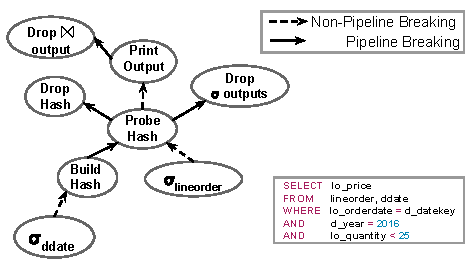
\includegraphics[width=\columnwidth]{figures/QueryPlan.pdf}
	\vspace*{-2em}
	\caption{A join query and its DAG}
	\label{fig:dag}
%	\vspace*{-1.5em}
\end{figure}

The Query Manager uses a DAG Traversal algorithm (cf. Algorithm~\ref{alg:dag-traversal}) to process the DAG, which essentially is an iterative graph traversal method. 
The algorithm simply finds nodes in the DAG that have all their dependencies met, and marks such nodes as ``active'' (line~\ref{alg:depMet}).
Work orders are requested and scheduled for all active nodes (line~\ref{alg:getWork}), and 
the completion of work orders is monitored. 
Operators are stateful and they produce work orders when they have the necessary data.
The work order generation stops (line~\ref{alg:finishGenWork}) when the operators no longer have any input to produce additional work orders.
When no more work orders can be generated for a node, that node is marked as 
``completed'' (line~\ref{alg:nodeComplete}). 
When a node is marked as completed, all outgoing blocking edges (the solid lines 
in Figure~\ref{fig:dag}) are ``activated'' (line~\ref{alg:outEdgesActive}). 
Pipelining is achieved as all non-blocking edges (dotted lines in 
Figure~\ref{fig:dag}) are marked as active upfront (line~\ref{alg:pipelining}).
The query is deemed as completed when all nodes are marked as ``completed.''

% Note(harshad) - The DAG traversal example seems to be taking lots of space and can be omitted, as it diverts the attention away from the meat of the paper. 
%\subsubsection{DAG Traversal Example}\label{sssec:dag-traversal-example}
%To illustrate the execution of the scheduler algorithm, consider the 
%DAG shown in Figure~\ref{fig:dag}.
%Initially, only the two selection relational operators (shown in the DAG using
%the symbol $\sigma$) are \textit{schedulable}.\footnote{Initially, the print 
%operator is \textit{active} too, but as there's no input available, it can't
%produce any work order.}
%So, the Query Manager generates work orders for these operators. 
%In this case, there is one work order for each input block in each of the two
%input relations.\footnote{To avoid both select operators from being co-scheduled
%concurrently, a dependency link can be created between these two operators.
%Thus, work on the select operator on the $\mathtt{lineorder}$ table is started
%only after the select operator on the $\mathtt{ddate}$ table has completed. 
%Such decisions are made by the optimizer.}
%
%The Foreman assigns these work orders to the available worker threads. 
%The worker threads execute the operations specified in the work orders. 
%Note that given the independent block design (see Section~\ref{ssec:storage-manager}) 
%it is possible that two work orders on the same table may invoke different code paths. 
%For example one block on the \verb+ddate+ table may have an index sub-block on 
%the \verb+d_year+ attribute, and this index may be chosen to evaluate the tuples 
%in that block. 
%Another block on that same \verb+ddate+ table may not have any indices, and so 
%the selection operation for tuples in that second sub-block may resort to a simple scan. 
%In addition, the operator algorithm may choose to make a local decision on which 
%access plan to use. 
%So, e.g. even if each data block in the \verb+ddate+ table has an index 
%of the \verb+d_year+ attribute some work orders may use the index and others may 
%not. (The optimization algorithm for making these local decisions is beyond the 
%scope of this paper.)
%Essentially, the scheduler is largely oblivious to how the work orders are executed 
%and there is no global recipe that is imposed on the work orders that correspond 
%to a node in the DAG.
%
%Work orders may produce output data that are stored in blocks in the buffer pool. 
%In the case of the query in Figure~\ref{fig:dag}, the selection work orders on the \verb+ddate+
%table insert the selected tuples into data blocks that correspond to a new 
%temporary table. 
%%(the execution of the work orders is vectorized for efficiency). 
%These data blocks are pipelined to the next stage.\footnote{There is a 
%mechanism to allow multiple concurrent work orders from the same
%operator in the DAG to insert into a common output/temporary data
%block to avoid block internal fragmentation, and to facilitate early 
%pipelining. We omit these details.}
%In other words, as soon as there is a full block of tuples from applying the 
%selection operator on the \verb|ddate| table, a work order is created for the 
%\textit{build hash} operator. (Notice that the edge connecting the selection
%operator and the build hash operator permits data pipelining.)
%
%To begin the probe phase of the hash join, the building of the hash table must be 
%complete, as there is a pipeline-breaking dependency between the probe operator 
%and the build operator. 
%Thus, the DAG traversal algorithm only marks the probe hash operator node as 
%active when the build hash operator has completed. 
%Results from probing the hash table can be immediately pipelined to the print 
%operator.
%The drop operators ensure that intermediate data is dropped before the query is 
%deemed to have completed. 

\section{Thread Model}\label{apx:thread}
\sys{} currently runs as a single server process, with mutiple user-space threads. 
There are two kinds of threads. 
There is one \textit{Scheduler} thread, and a pool of \textit{Worker} threads. 
All the components in 
Figure~\ref{fig:scheduler-architecture} except the worker thread pool run in the 
scheduler thread. 
In the current implementation, all threads are spun upfront when the database server 
process is instantiated, and stay alive until the server process terminates.

The threads use the same address space and use shared-memory semantics for data 
access. 
In fact the buffer pool is stored in shared memory, which is accessible by all the threads. 
Each worker thread is typically pinned to a CPU core. 
Such pinning avoids costs incurred when a thread migrates from one CPU core to another, which results in loss of data and instruction cache locality. 
We do not pin the scheduler thread, as its CPU utilization is low and it is not worth dedicating a CPU core for the scheduler thread.

Every worker thread receives a work order from the Foreman, executes it and then waits for 
the next work order.
In order to minimize worker's idle time, typically each worker is issued multiple work 
orders at any given time. 
%When a work order is sent to a worker thread, it executes the work order.
 %the worker thread simply invokes %the appropriate \verb|execute()| method (described in~\ref{ssec:workorders}). 
Thread-safe queues are used to communicate between the threads.
%The communication happens through light-weight messages from the sender to the receiver thread, which is internally implemented as placing a message object on the receiver's queue. 
%A receiver reads messages from its queue. 
%A thread (and its queue) is uniquely identified by its thread ID. 

%The thread communication infrastructure also implements additional features 
%like the ability to query the lengths of any queue in the system, and cancellation 
%of an unread message. 
%For simplicity, we omit discussion of these aspects. 

\section{Policy Enforcer}\label{apx:policy-enforcer}
The Policy Enforcer applies a high level policy for resource allocation among concurrent queries. 
It uses a probabilistic-framework to select work orders from a pool of work orders 
belonging to different concurrent queries for scheduling. 
The Policy Enforcer assigns a probability to each active query, which indicates the likelihood of a work order from that query getting scheduled for execution in the near future. 
The probability-based work order selection strategy brings powerful control to the scheduler through a single parameter -- i.e. by controlling the probability 
setting, the scheduler can control the resource sharing among concurrent queries. 
%A work order from a query with higher probability is more likely to get scheduled 
%than a work order from a query with lower probability. 

The challenge in designing the policy enforcer lies in transforming the policy specifications to a set of probabilities. 
A critical piece that we use in such transformations is the prediction of work order 
execution times for the concurrent queries, which is done by the Learning Agent described in Section~\ref{ssec:learning}. %and depicted in Figure~\ref{fig:scheduler-cycle}.
In the remainder of this section, we provide an intuition for deriving probability values from the work order execution times. 
A formal model for the probability computations for different policies is presented in Section~\ref{sec:policy}.

\begin{figure}[]
	\centering
	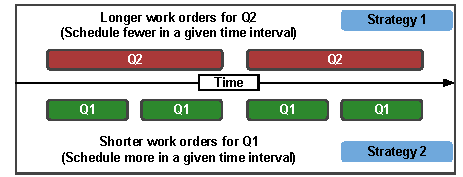
\includegraphics[width=\columnwidth]{figures/Probability-explanation.pdf}
	\vspace{-2em}
	\caption{Scheduling queries having different work order execution times for the fair policy. The solid boxes with $Q_{i}$ depicts the lifetime of a work order from the Query $Q_{i}$.}
	\label{fig:probability-explanation}
	%	\vspace{-1.5em}
\end{figure}

We now motivate the probabilistic approach used by the Policy Enforcer with an example.
Consider a single CPU core and two concurrent queries $q_{1}$ and $q_{2}$. 
(The idea can be extended to multi-cores and more than two queries.)
Initially, we assume perfect knowledge of the execution times of work orders of the queries. 
Later, we will relax this assumption. 

Let us assume that as per the policy specifications, in a given time interval, the CPU resources should be shared equally. 
Suppose that work orders for $q_{1}$ take less time to execute than work orders for 
$q_{2}$, as shown in Figure~\ref{fig:probability-explanation}.
As the Policy Enforcer aims to allocate equal share of the CPU to $q_1$ and $q_2$, a simple strategy can be to schedule proportionally more work orders of $q_{1}$  than those of $q_{2}$, in a given time window. 
The number of scheduled work orders is inversely related to the work order execution 
time. 
This proportion can be determined by the probabilities $pb_{1}$ and $pb_{2}$ for queries $q_1$ and $q_2$, respectively.
The probability $pb_i$ is the likelihood of the scheduler scheduling next work order from query $i$. 
The probability is assigned by the Policy Enforcer to each active query in the system.
Note that, $pb_{1} > pb_{2}$ and $pb_{1} + pb_{2} = 1$.

%Such strategy will result in similar \textit{CPU occupancy} with respect to time 
%for both the queries, thereby fairly sharing the CPU resource in a given time 
%frame.  If the policy enforcer keeps scheduling the work orders similarly for the rest of 
%the  workload execution, it is easy to see that the queries will share the CPU 
%\textit{fairly}, as demanded by the policy. 

Notice that the Policy Enforcer is not concerned with the complexities of the operators in the query DAGs. 
It simply maintains the probability associated with each active query which is determined by the query's predicted work order execution times.

The Policy Enforcer can also function with workloads that consist of queries categorized in multiple classes, where each class has a different level of ``importance'' or ``priority''. 
The policy specifies that the resource allocation to a query class must simply be in accordance to its importance, i.e. queries in a more important class should collectively get a higher share of the resources, and vice versa.
In such scenarios, the Policy Enforcer splits its work order selection strategy in two steps - selection of a query class and subsequent selection of a 
query within the chosen query class.
Intuitively, the Policy Enforcer should assign higher probability to the more 
important class and lower probability to the less important class.

Once a query class is chosen, the Policy Enforcer must pick a query from the chosen class. 
Each query class can specify an optional intra-class resource allocation sub-policy. 
By default, all queries within a class are treated equally.
Thus, the probability-based paradigm can be used to control both inter and intra-class resource allocations.

There could be many reasons for categorizing queries in classes, including the need to associate some form of urgency (e.g. interactive vs batch queries), or marking the importance of the query source 
(e.g. the position of the query submitter in an organizational hierarchy). 
In addition, the resource allocations across different classes can also be chosen based on various scales, such as linear or exponential scale allocations based on the class number. 
An attractive feature of the Policy Enforcer is that it can be easily configured for use in a variety of ways.
Under the covers, the Policy Enforcer simply maps each class to a collective class probability value, and then maps each query in each class to another probability. 
Once these probabilities are calculated, the remaining mechanisms simply use them to appropriately allocate resources to achieve the desired policy goal.

\section{Motivation for the Learning Agent Module}\label{apx:learning-motivation}
One might question the need of the Learning Agent and instead consider assigning a fixed probability value to each query (say $1/N$, with $N$ queries in the fair policy).
In the following section, we address this issue. 
A motivational example for the learning agent is described in Appendix~\ref{apx:learning-motivation}.

We perform an experiment, where the goal is to analyze the patterns in work order execution times of two queries. 
The dataset used for the experiment comes from the Star Schema Benchmark (SSB)~\cite{ssb} 
at a scale factor of 100 (c.f. Section~\ref{ssec:workload} for benchmark details).
We pick two SSB queries $Q1.1$ and $Q4.1$, and execute them on a machine with 40 CPU cores. 
$Q1.1$ has a single join operation and $Q4.1$ has four join operations.
Figure~\ref{fig:q1.1-q4.1-time-per-wo} shows the observed average time per work order for both queries.
We now describe the trends in time per work order for the queries.

We can observe $Q1.1$'s execution pattern denoted by the dashed line in Figure~\ref{fig:q1.1-q4.1-time-per-wo}. 
The time per work order remains fairly stable (barring some intermittent fluctuations) from the beginning until 1.8 s.
This phase corresponds to the selection operation in $Q1.1$ which evaluates predicates on the \textit{lineorder} (fact) table.
A small bump in time per work order can be observed at the 1.8 s mark, when the probe phase of $Q1.1$ begins and continues until 2 s.
Towards the end of the execution of $Q1.1$, (2.2 s) there is a spike in time per work order when the query enters the aggregation phase. 
The output of the hash join is fed to the aggregation operation. 
The results of aggregation are stored in per-thread private hash tables, which are later merged to produce the final output.

\begin{figure}[h]
	\centering
	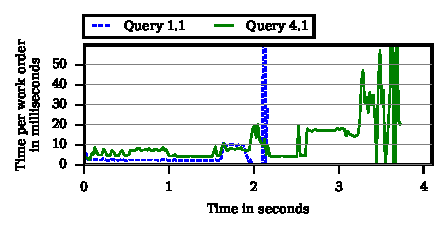
\includegraphics[width=\columnwidth]{figures/q11-q41-time-per-wo.pdf}
	\vspace{-2.5em}
	\caption{Time per work order for Q1.1 and Q4.1}
	\label{fig:q1.1-q4.1-time-per-wo}
%	\vspace{-2em}
\end{figure}

Now we analyze the execution pattern for $Q4.1$ which has 4 join operations. 
This query is more complex than $Q1.1$.% which has a single join.
%Due to the more complex nature of the query, 
Therefore, the execution pattern of $Q4.1$ exhibits more phases, with different times per work order as compared to $Q1.1$.
Various small phases before the 0.5 s mark correspond to the selection predicates that are applied to the dimension tables. (Note that in $Q4.1$ there is no selection filter on the \textit{lineorder} table).
The selections on dimension tables get executed quickly.
The longer phases denote the different probe hash table operations in the query.
Towards the end, similar to $Q1.1$, there is a spike in the execution time per work order which correspond to the aggregation phase.

It is clear that the work order execution times for both queries are different, and the difference between them changes over time. 
If the scheduler assigns the same probability to both queries (i.e. 0.5), it is equally likely to schedule a work order from either of them. 
As a result, the queries will have different CPU utilization times in a given epoch, thus resulting in an unfair CPU allocation. 
In order to be consistently fair in allocating CPU resources to the queries, we should continuously observe the work order execution times of queries and adjust the CPU allocation accordingly. 

\section{Storage Management in \sys{}}\label{apx:storage-manager}
Data organization in the \sys{} storage manager holds the key to intra-query 
parallelism~\cite{qsstorage}. 
Data in a relation are organized in the form of blocks. 
Each block holds a collection of tuples from a single table. 
A unique aspect of the storage organization in \sys{} is that blocks are considered to 
be independent and self-contained mini-databases. 
Thus, when creating an index, instead of creating a global index with 
``pointers'' to the tuples in blocks, the index fragments are stored within the blocks. 
Each block is internally organized into \textit{sub-blocks}. 
There is one \textit{tuple storage sub-block}, which could be in a row store or a 
column store format.
%\reminder{Should we add more formats like compressed column store etc?}. 
In addition, each block has one sub-block for each index created on the table. 
CSB+-tree~\cite{csb+-tree} and BitWeaving~\cite{bitweaving} 
indices are currently supported. 
The blocks are free to self-organize themselves and thus a given table may have blocks in different formats. 
For example, new blocks in a table may be in a row store format, while older blocks may 
be in a column store format.
%The block size is configurable %(in fact blocks in the same table can be of 
%%different sizes), %and the recommended block size is 4 MB.

This storage block design, as articulated earlier in~\cite{qsstorage} enables the query execution to be broken down into a set of independent tasks on each block. 
This is a crucial aspect that we leverage in the design of our scheduler. 

% Note(harshad) - The following paragraph seems too much information, hence removing it. 
%The storage manager also contains a \textit{buffer pool manager}. 
%It organizes the memory as an array of slots, and overlays blocks on top of the slots (so block sizes are constrained to be a multiple of the underlying slot size). 
%Memory allocations for data blocks for \textit{both} permanent and temporary tables are always made from a centralized buffer pool. 
%In addition, all allocations for run-time data structures, such as hash tables are also made 
%by the buffer pool. 
%The buffer pool manager employs an LRU-2~\cite{lruk} replacement policy. 
%Thus, it is possible for a hash table to get evicted to disk, if it has become ``cold''; e.g. if it belongs to a suspended query.

\section{Resource Map Discussion}\label{apx:resource-map}
An example Resource Map of an incoming query to the system is shown below:
\begin{lstlisting}[language=python, 
								   basicstyle=\ttfamily\small, 
								   showstringspaces=false,
								   keywordstyle=\color{bondiblue}\bfseries, 
								   emph={CPU, Memory}, 
								   emphstyle=\color{cardinal}\bfseries]
CPU:    {min: 1 Core, max: 20 Cores}
Memory: {min: 20 MB,  max: 100 MB}
\end{lstlisting}

This Resource Map states that the query can use 1 to 20 cores (i.e. specifies the range of intra-operator parallelism) and is estimated to require a minimum of 20 MB of memory to run, and an estimated 100 MB of memory in the worst case.

In \sys{}, the query optimizer provides the estimated memory requirements for a given query.
Other methods can also be used, such as inferring the estimated resources from the previous runs of the query or other statistical analyses.
The scheduler is agnostic to how these estimates are calculated.

\section{Pipelining in \sys{}}\label{apx:pipelining}
During a work order (presumably belonging to a producer relational operator in a pipeline) execution, output data may be created (in blocks in the buffer pool). 
When an output data block is filled, the worker thread sends a ``block filled'' message to the corresponding query's manager via the following channel: Worker $\rightarrow$ Foreman $\rightarrow$ Policy Enforcer $\rightarrow$ Query Manager.
The Query Manager may then create a new work order (for a consumer relational operator in the pipeline) based on this information;
e.g. if this block should be pipelined to another operator in the query plan.

Note that pipelining in \sys{} works on a block-basis, instead of the traditional tuple-basis.

\section{Resource Choices for Policy Implementations and Load Controller Implementations}\label{apx:resource-discussion}
In the current implementation of \sys{}, we have focused on two key types of resource in the in-memory deployment scenarios -- CPU and memory. 
Both these resources have different resource characteristics, which we outline below.

First, consider the CPU resource. 
On modern commodity servers there are often tens of CPU cores per socket, and the aggregate number of cycles available per unit time (e.g. a millisecond) across all the cores is very large. 
Further, an implication of \sys{}'s fine-grained task allocation and execution paradigm is that the CPU resource can be easily shared at a fine time-granularity. 
Several work orders, each from different query can be executed concurrently on different CPU cores, and each query may execute thousands or millions or even more number of work orders. 
Thus, in practical terms, the CPU resource can be viewed as a nearly infinitely divisible resource across concurrent queries. 
In addition, overall system utilization is often measured in terms of the CPU utilization. Combining all these factors, specifying a policy  in terms of the CPU utilization is natural, and intuitive for a user to understand the policy. 
For example, saying that a fair policy equally distributes the CPU resource across all (admitted) concurrent queries is simple to understand and reason. 

Memory, on the other hand, is a resource that is allocated by queries in larger granular chunks. 
Active queries can have varying memory footprints (and the footprint for a query can change over the course of its execution). 
Thus, memory as a resource is more naturally viewed as a ``gating'' resource. 
Therefore, it is natural to use it in the load controller to determine if a query can be admitted based on its requested memory size. 
Actual memory consumption for queries can also be easily monitored, and when needed queries can be suspended if memory resource needs to be freed up (for some other query, perhaps with a higher priority). 

\section{Usage of Linear Regression in Learning Agent}\label{apx:linear-regression-usage}
The Learning Agent uses linear regression for predicting the execution time of the future work orders.
To lower the CPU and memory overhead of the model, we limit the amount of execution statistics stored in the Learning Agent.
We discard records beyond a certain time window. 
When all the work orders of an operator finish execution, we remove its records completely. 
In a query, if multiple relational operators are active, linear regression combines the statistics of all active operators and predicts a single value for the next work order execution time.

\section{Applicability of SSB for our evaluation}\label{apx:ssb}
The SSB is based on the TPC-H benchmark, and is designed to measure the query performance when %database systems in support of classical 
the data warehouse uses the popular Kimball~\cite{Kimball} approach. 
At a scale factor of X, the benchmark corresponds to about X GB of data in the 
corresponding TPC-H warehouse.
The SSB benchmark has 13 queries, divided in four categories. 
Each query is identified as \textbf{qX.Y}, where $X$ is the class and $Y$ is the query 
number within the class.
There are four query classes. 
, i.e. $1\leq X\leq4$. 
The first and second classes have three queries each, the third class has four queries, and 
the fourth class has three queries.
The queries in each category are similar with respect to aspects such as the 
number of joins in the query, the relations being joined, the filter and aggregation 
attributes. 
The grouping of queries in various classes makes this benchmark suitable for our 
experiments, as it provides a way of assigning priorities to the queries based on their class. 
	

%\end{thebibliography}

% that's all folks
\end{document}
